% Copyright 2021 Joel Feldman, Andrew Rechnitzer and Elyse Yeager, except where noted.
% This work is licensed under a Creative Commons Attribution-NonCommercial-ShareAlike 4.0 International License.
% https://creativecommons.org/licenses/by-nc-sa/4.0/


 \begin{frame}{Table of Contents }
\mapofcontentsB{\bc}
 \end{frame}
%----------------------------------------------------------------------------------------
%----------------------------------------------------------------------------------------
\section{2.3 Centre of Mass}
%---------------------------------------------------------------------------------------
%----------------------------------------------------------------------------------------
%----------------------------------------------------------------------------------------
\begin{frame}[t]
\label{note2.3a}
\StatusBar{1}{6}
\begin{block}{Centre of Mass}If you support a body at its centre of mass (in a uniform gravitational
field) it balances perfectly. That's the definition of the centre of mass
of the body.\end{block}
\begin{center}
\begin{tikzpicture}
\draw[ultra thick] (-4,0)--(4,0);
\onslide<-4>{\draw (-3,0)node[above,inner sep=0]{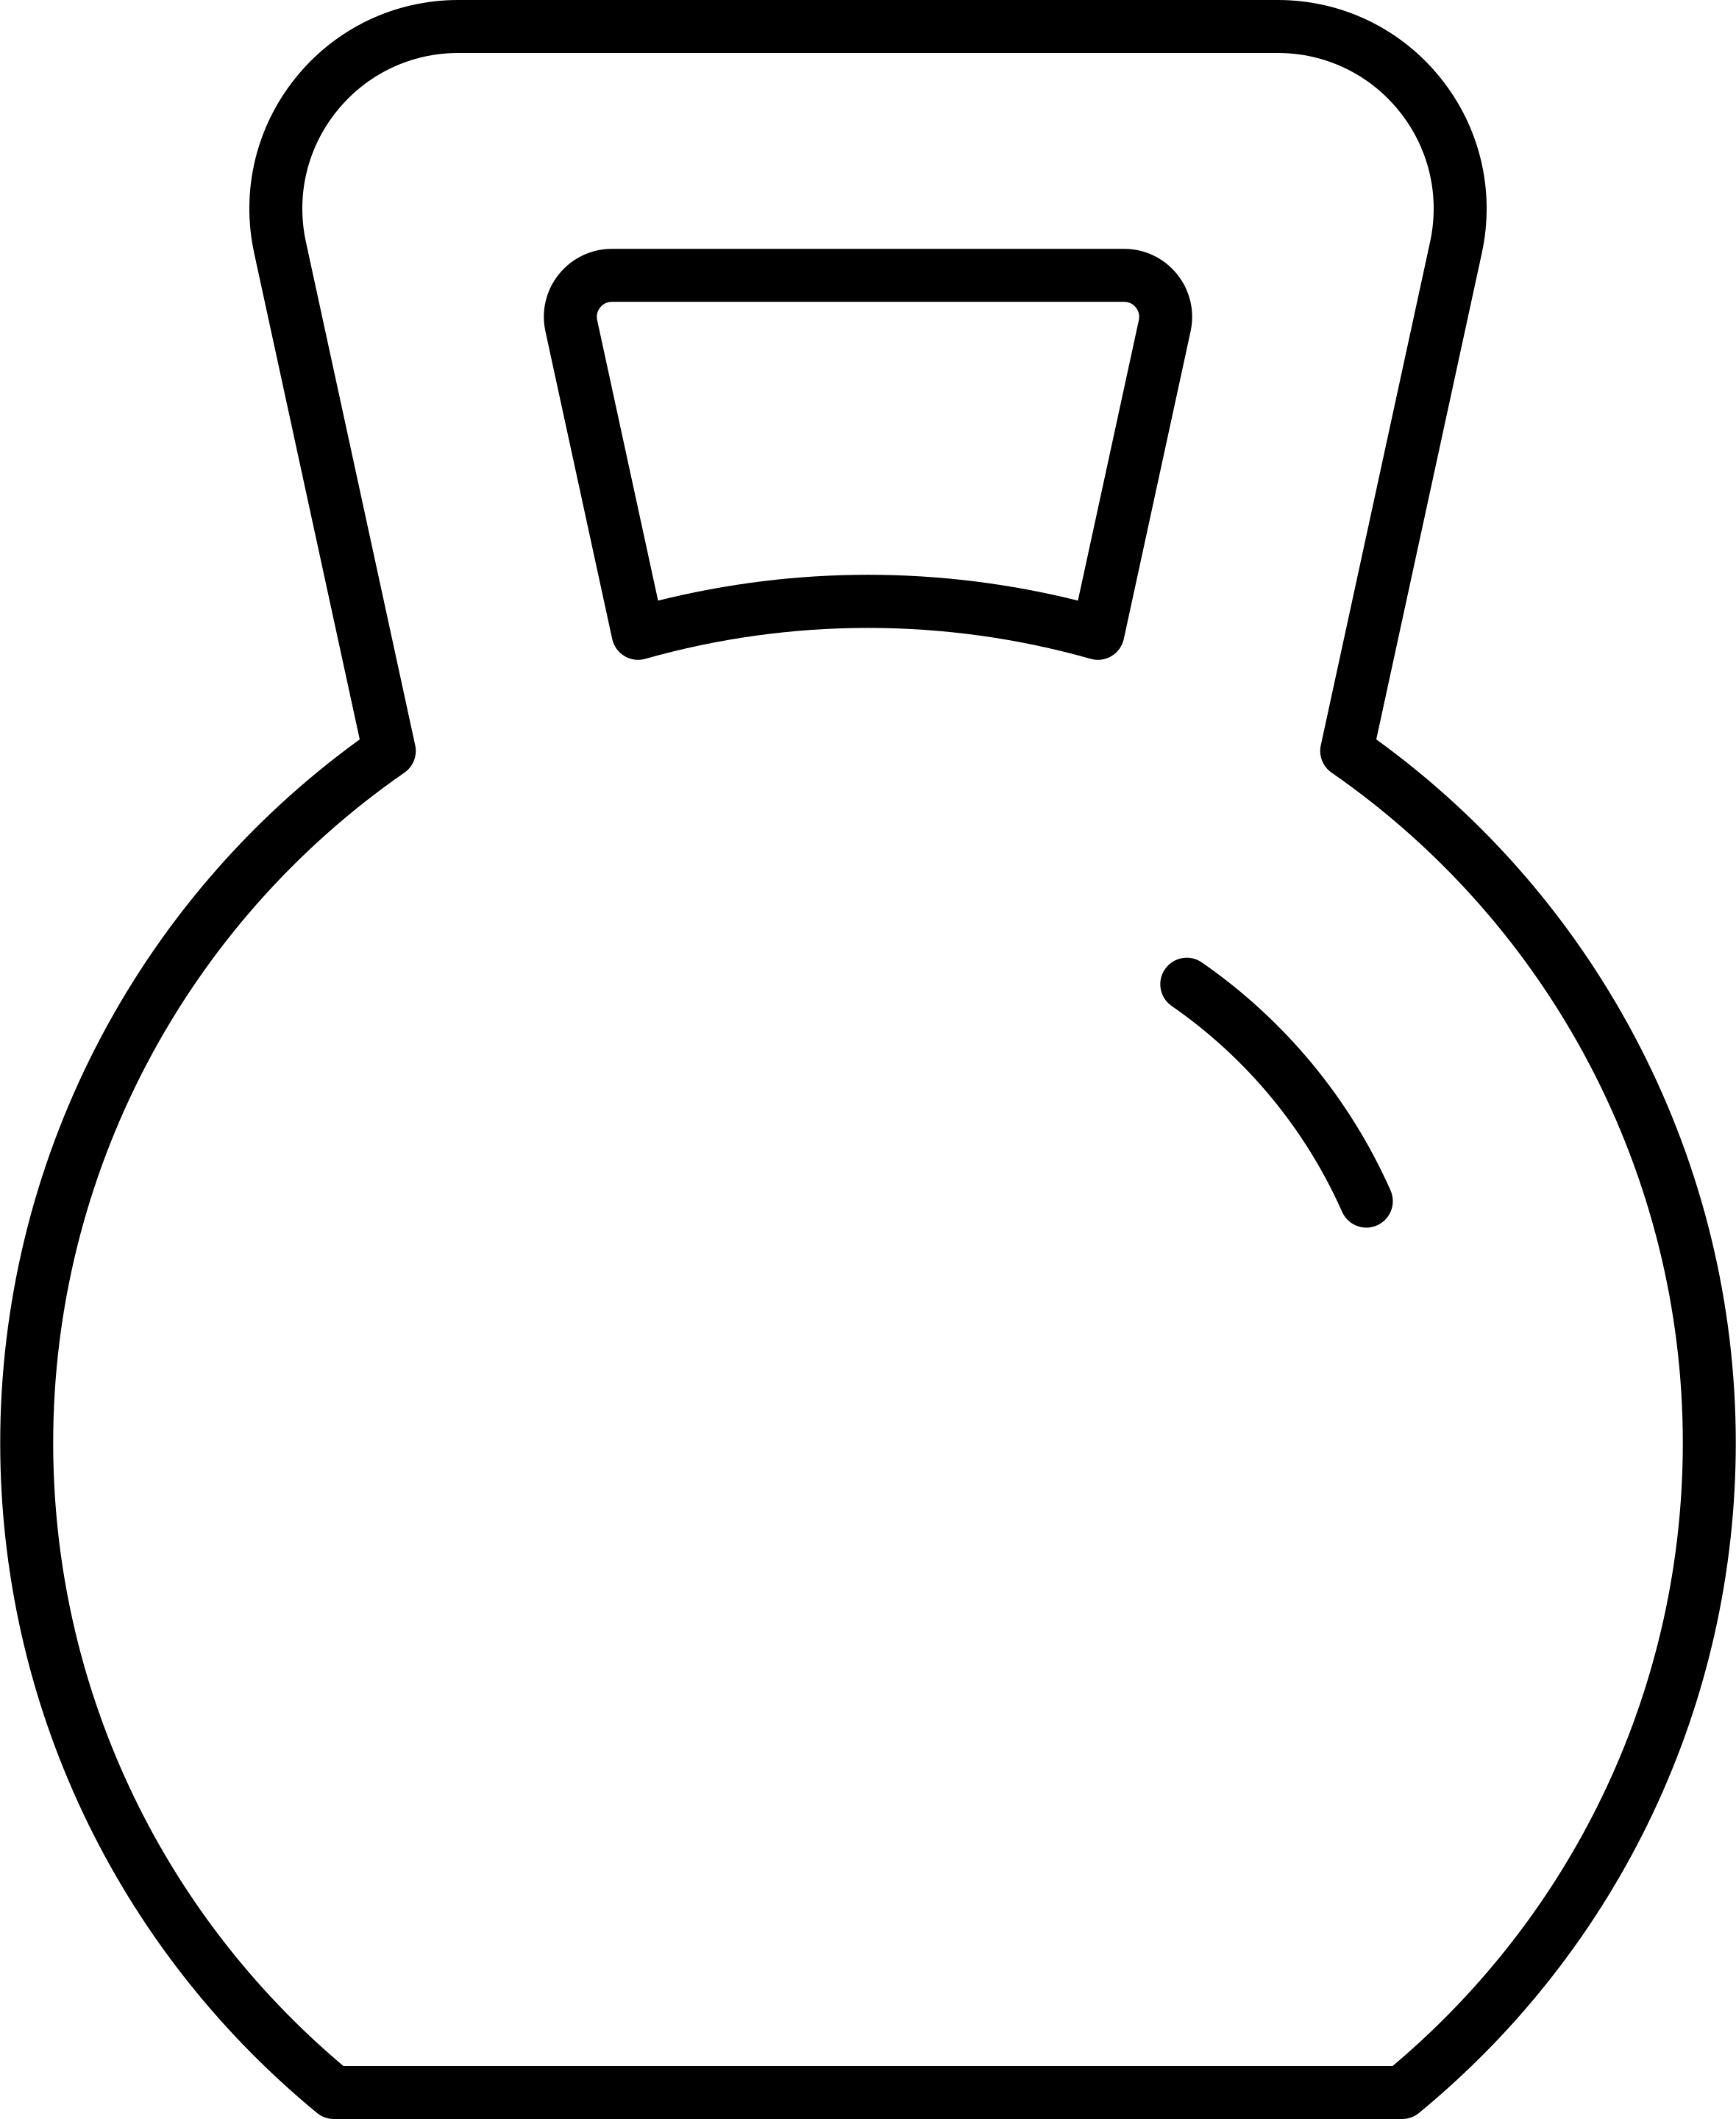
\includegraphics[width=1cm]{clipart/kettlebell}};
\draw (-3,.25)node{1 kg};}
\draw (3,0)node[above,inner sep=0]{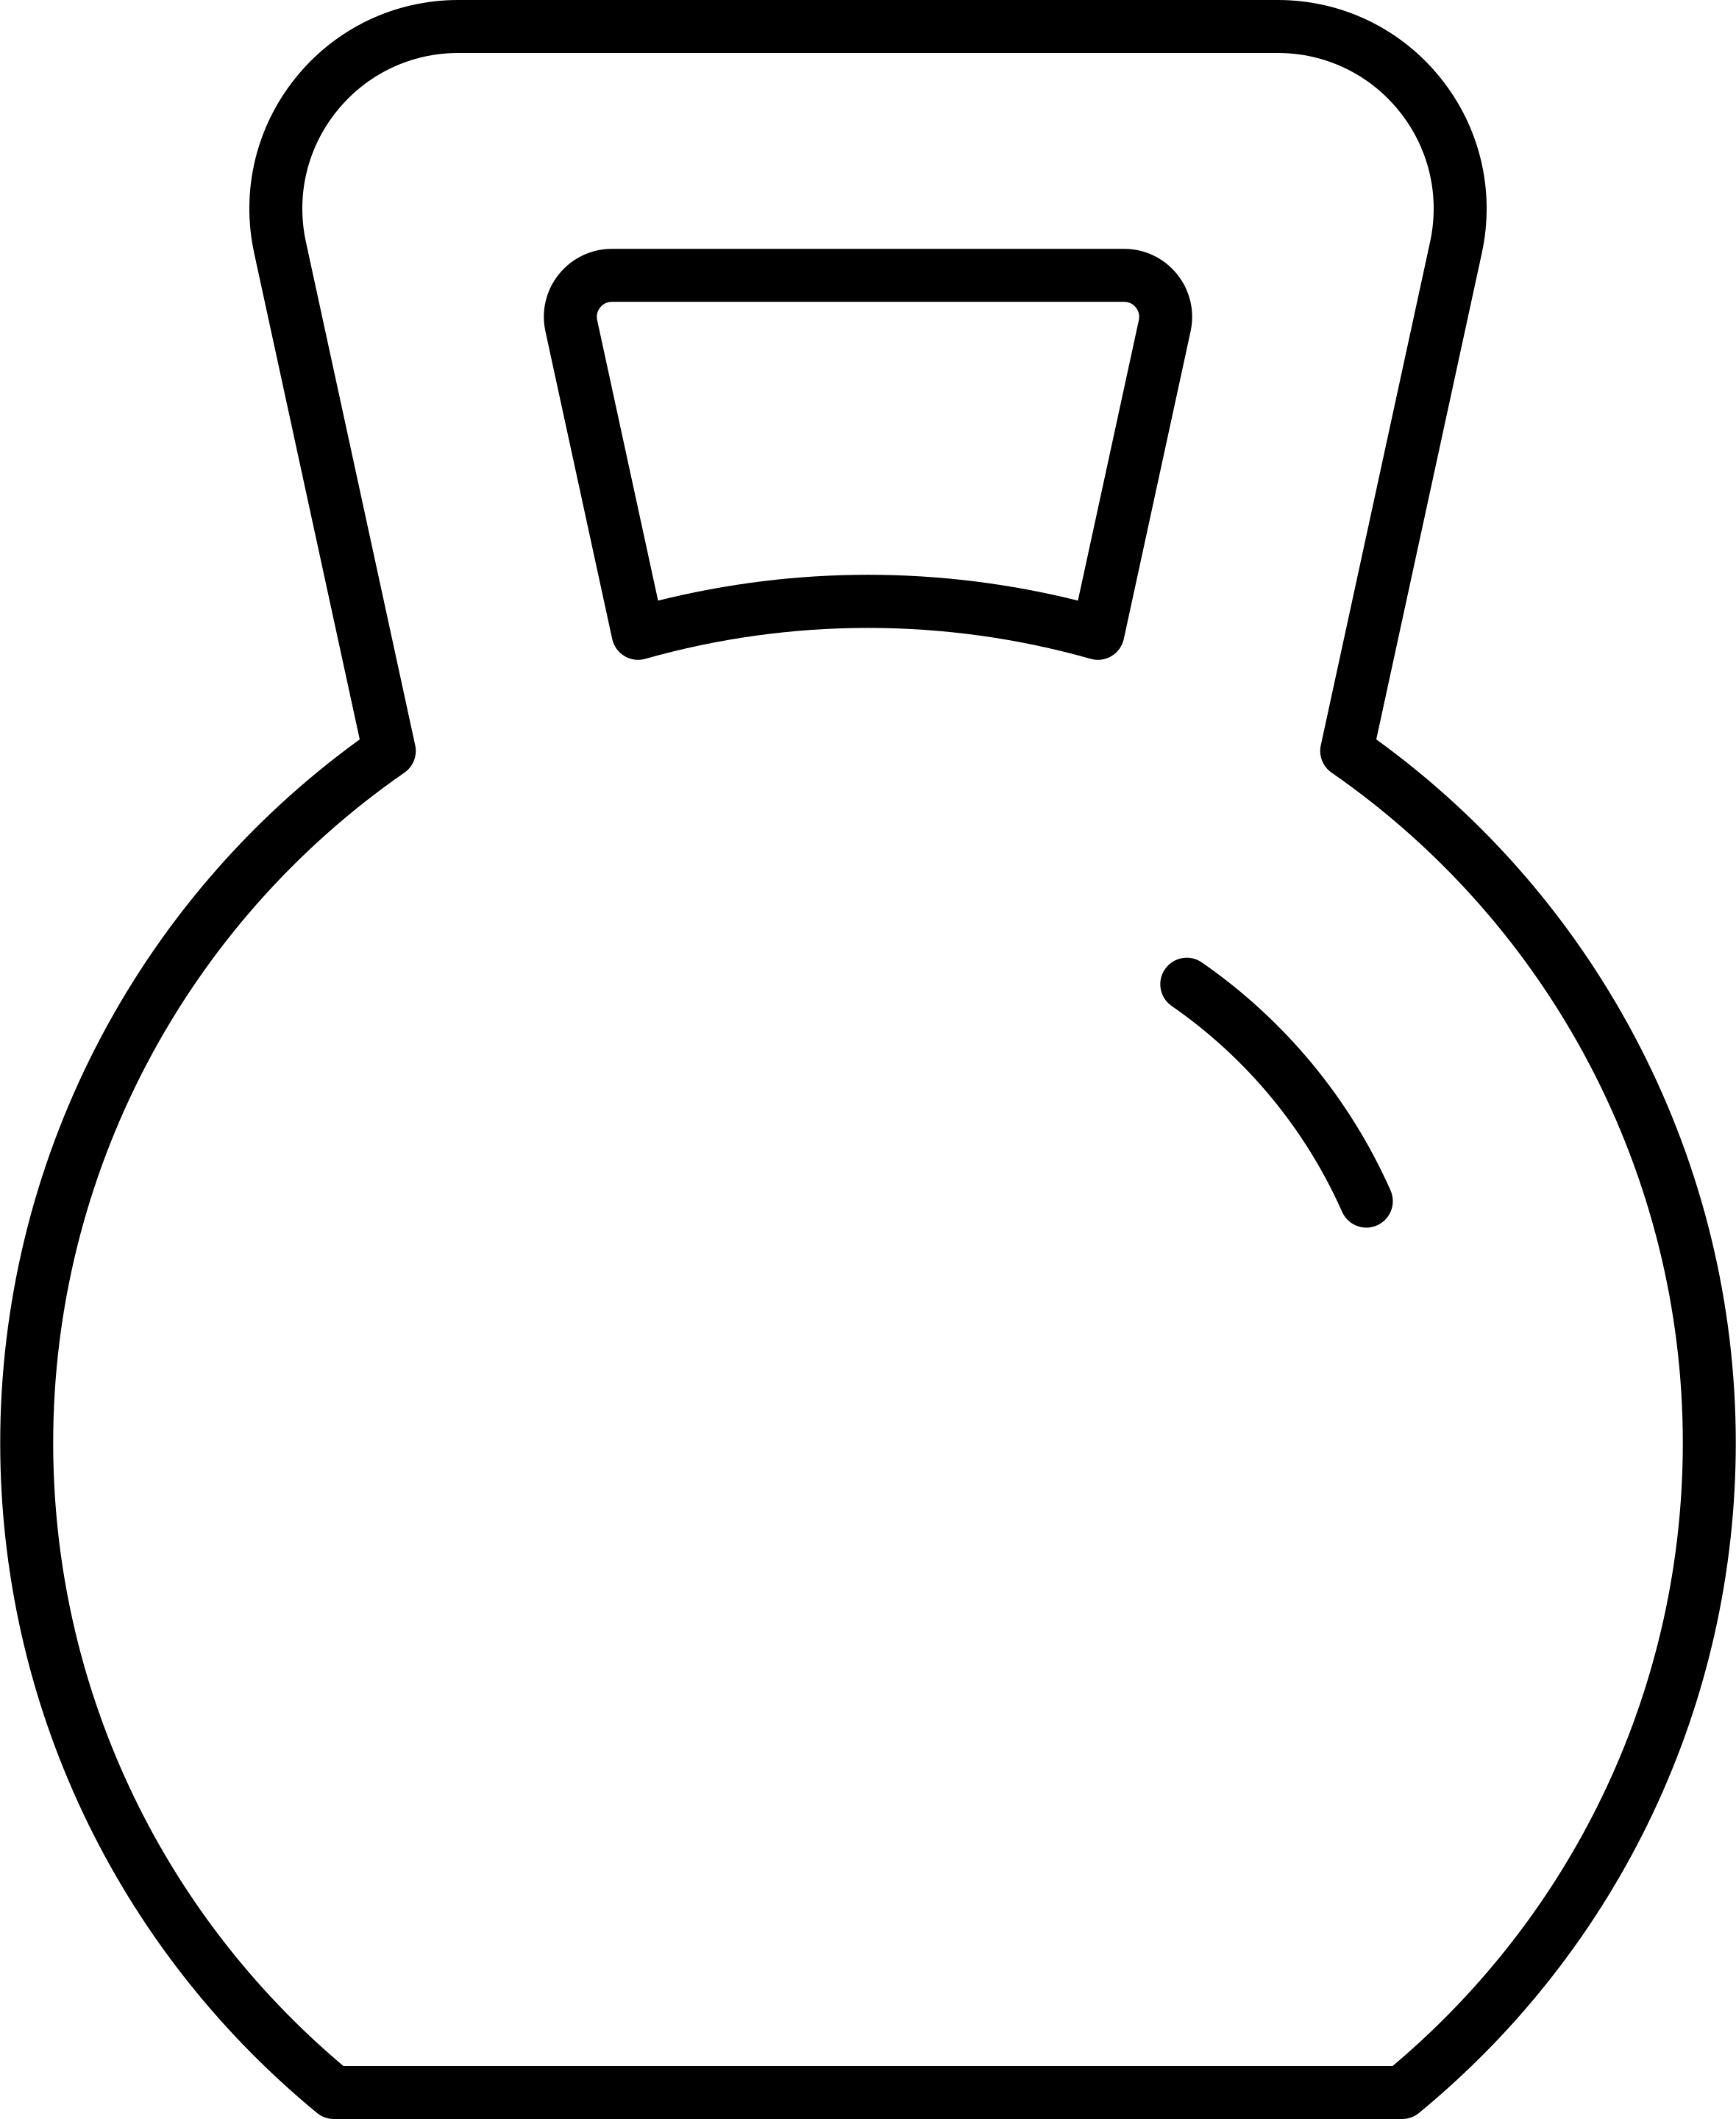
\includegraphics[width=1cm]{clipart/kettlebell}};
\draw (3,.25)node{1 kg};
\onslide<2>{\filldraw[C3] (0,0)--(-.5,-.5)--(.5,-.5)--cycle;}

\onslide<3-|handout:0>{
\draw (1,0)node[above,inner sep=0]{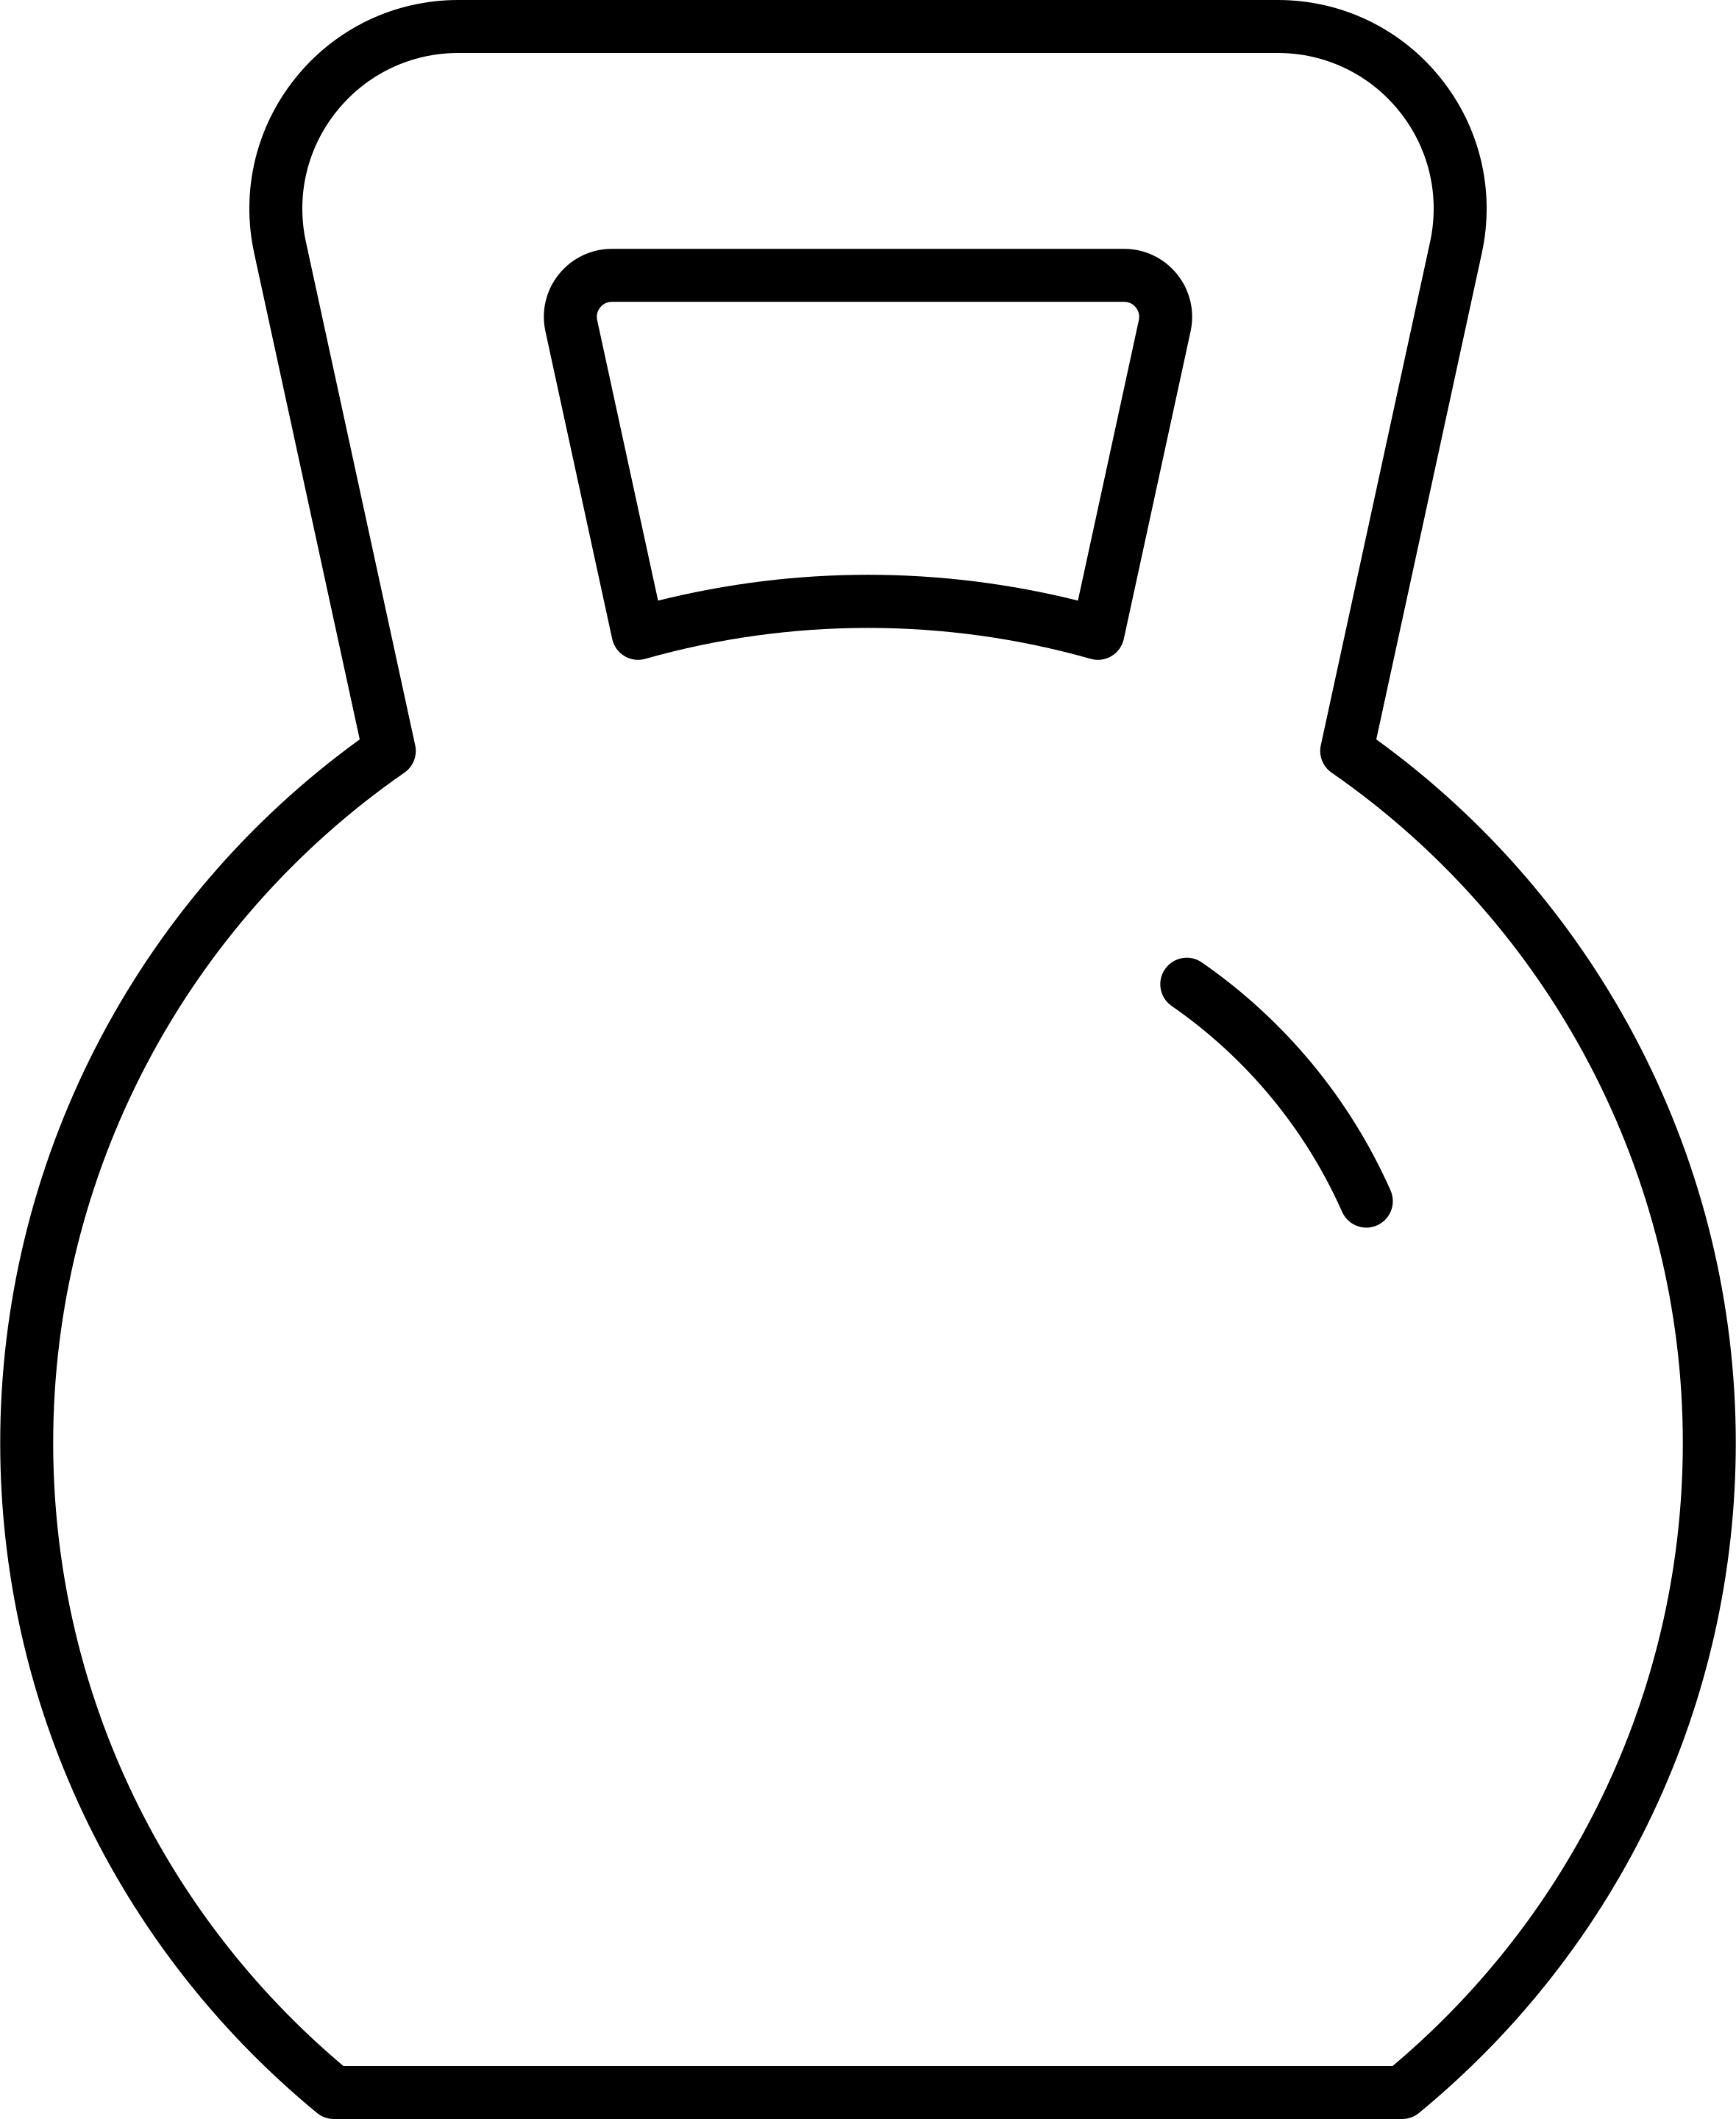
\includegraphics[width=1cm]{clipart/kettlebell}};
\draw (1,.25)node{1 kg};	
	}
\onslide<4|handout:0>{\filldraw[C3,xshift=0.33 cm] (0,0)--(-.5,-.5)--(.5,-.5)--cycle;}

\onslide<5-|handout:0>{\draw (-3,0)node[above,inner sep=0]{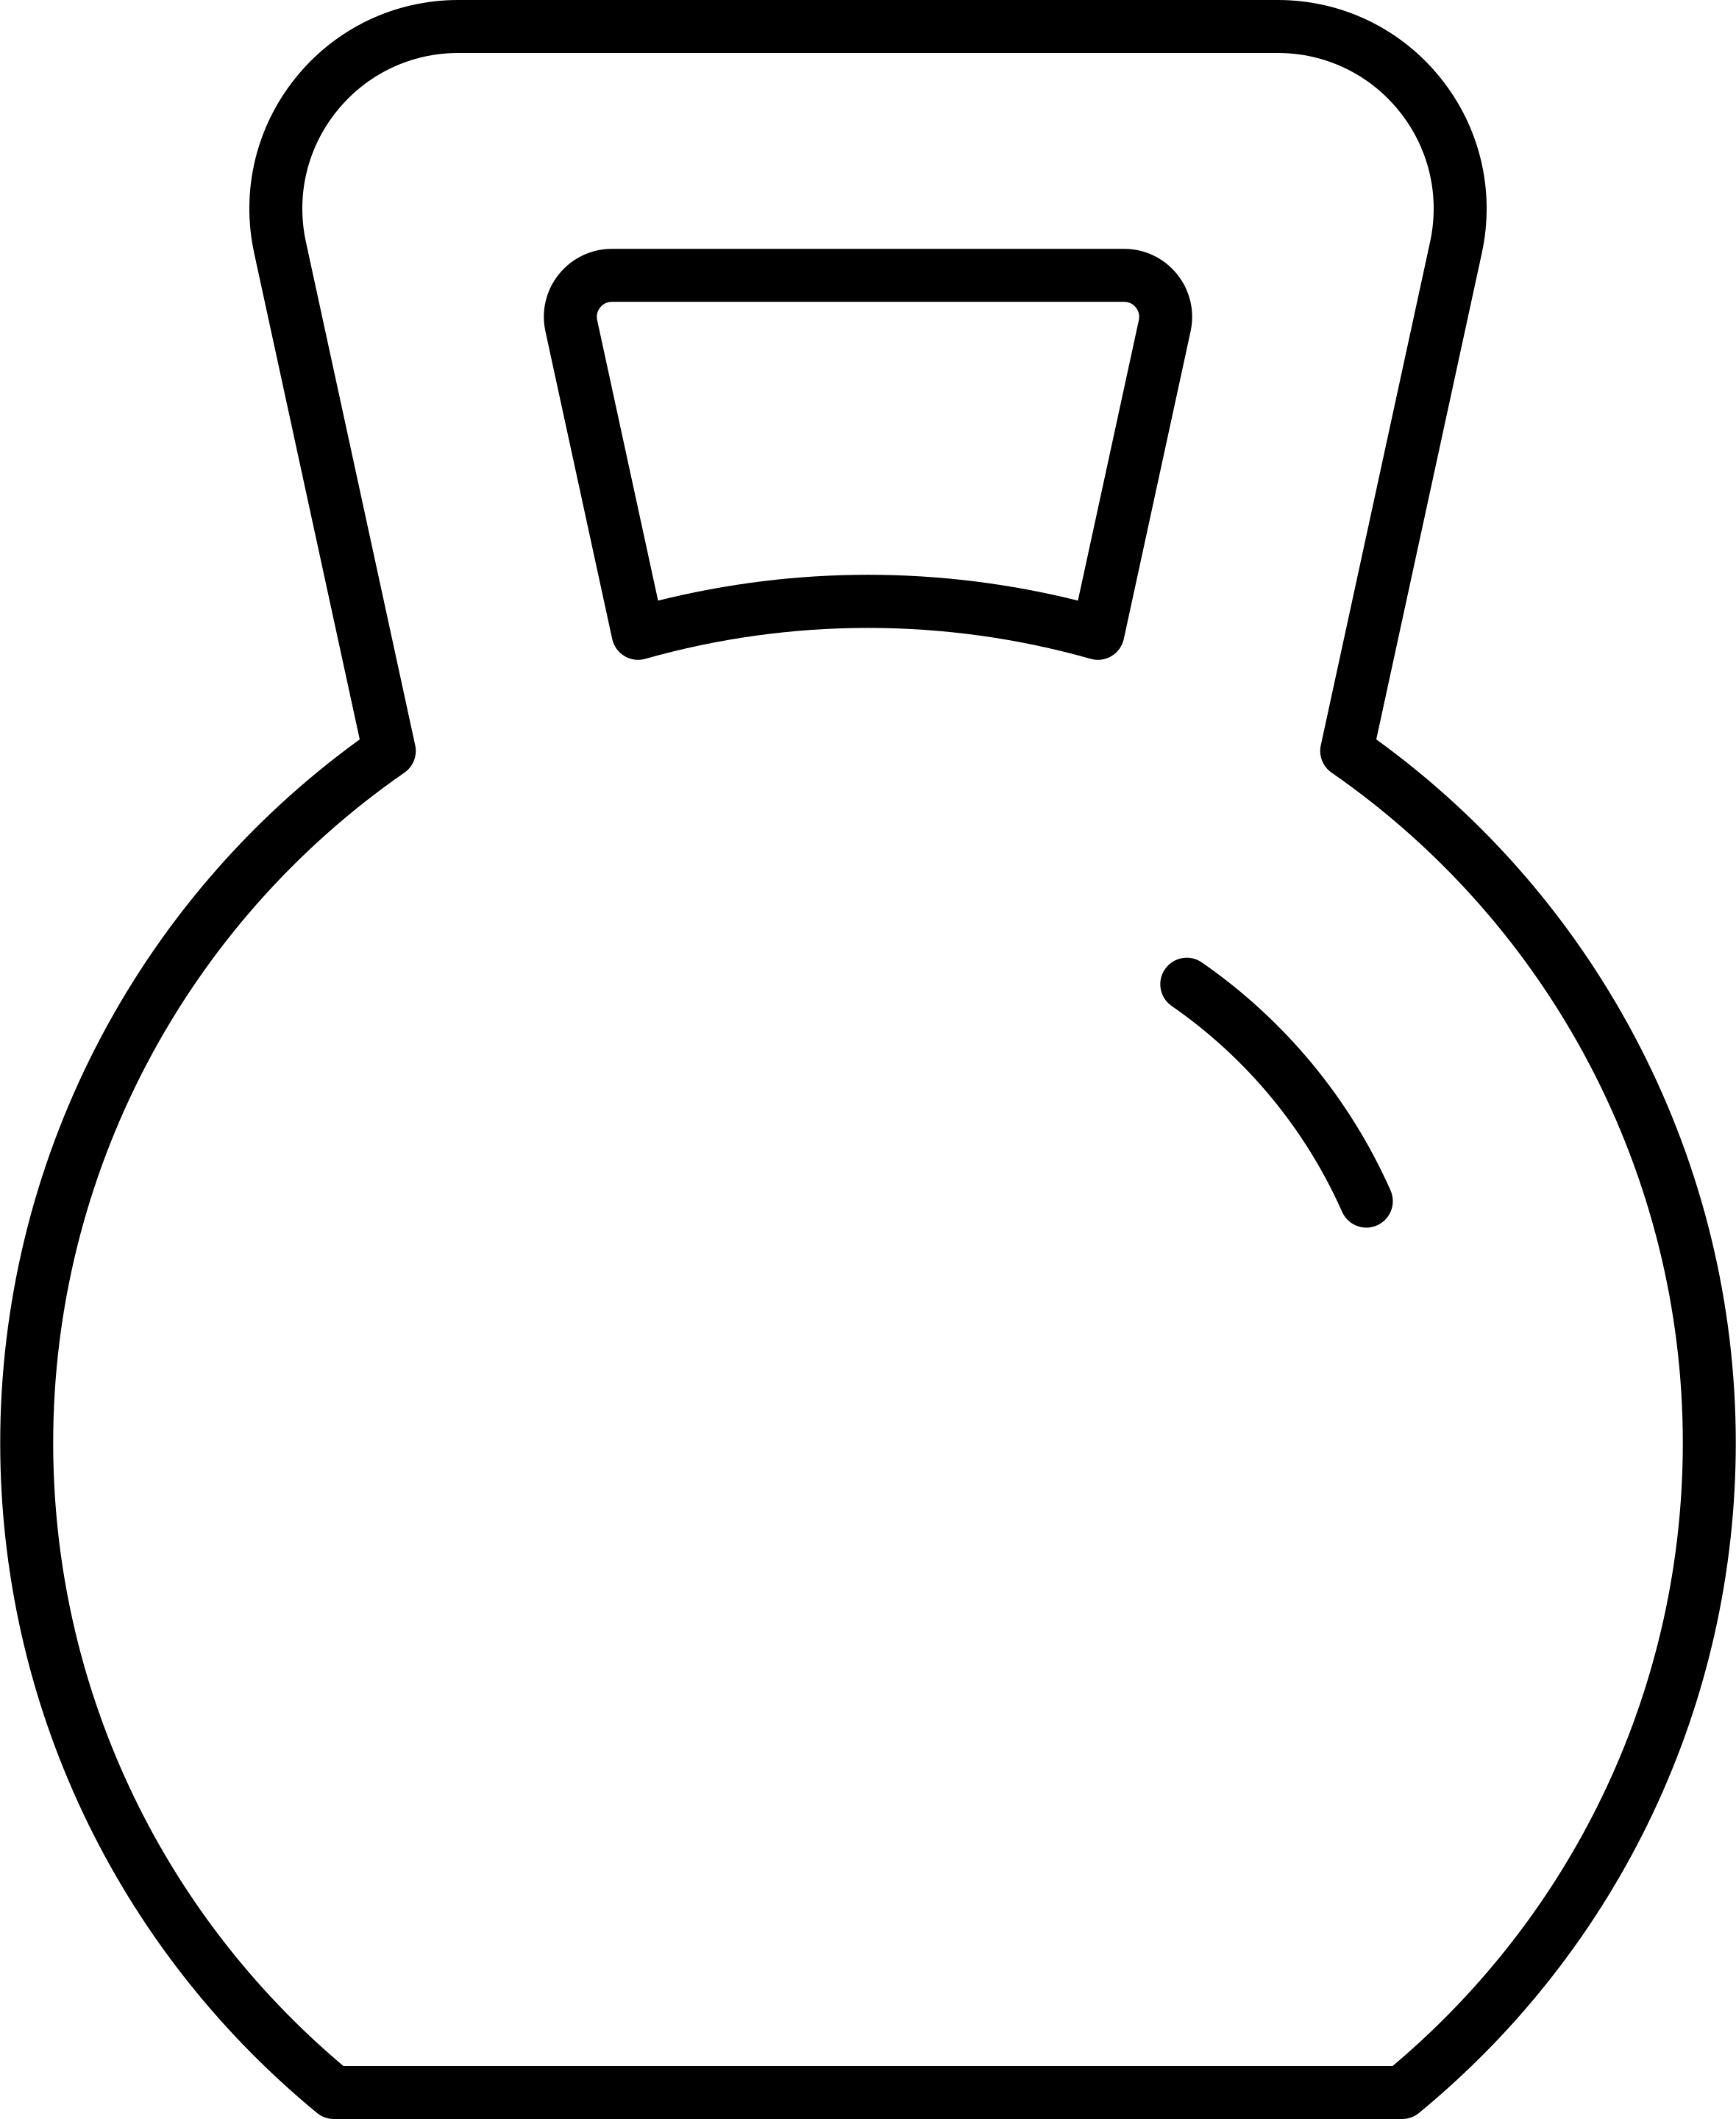
\includegraphics[width=1.5cm]{clipart/kettlebell}};
\draw (-3,.25)node{10 kg};}
\onslide<6|handout:0>{\filldraw[C3,xshift=-2.16 cm] (0,0)--(-.5,-.5)--(.5,-.5)--cycle;}
\end{tikzpicture}
\end{center}
\index{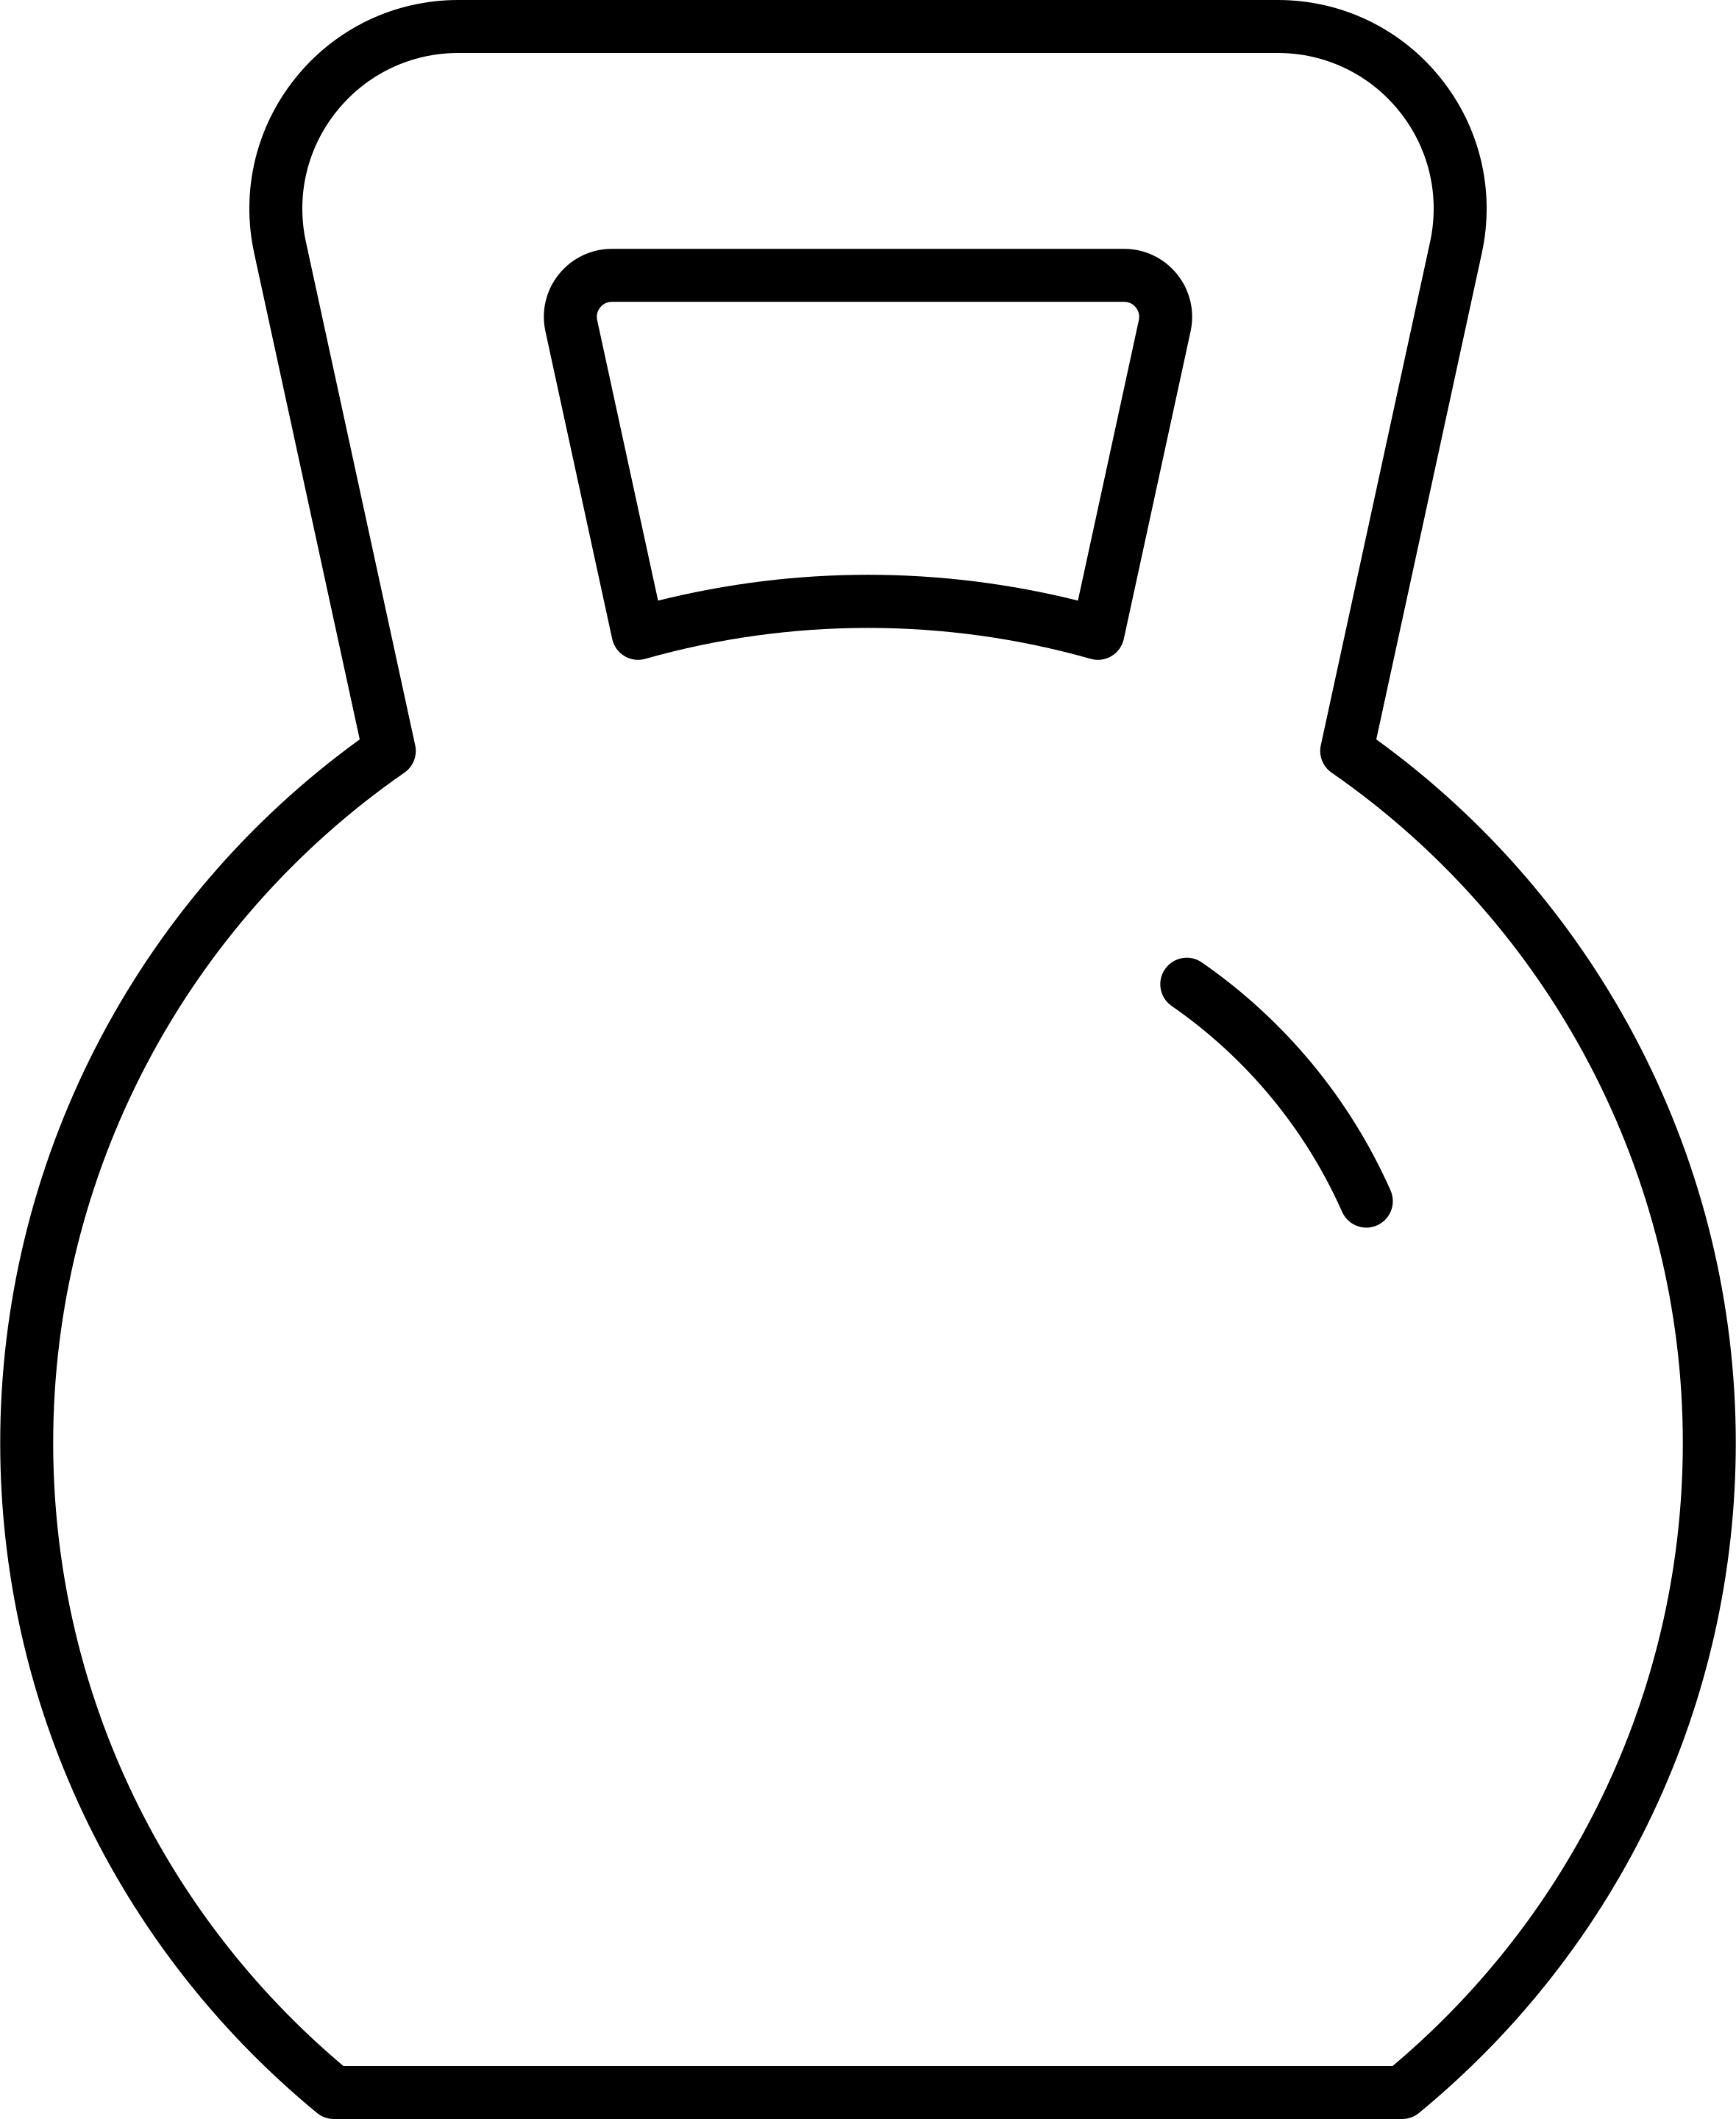
\includegraphics[height=3mm]{clipart/kettlebell} \href{https://thenounproject.com/icon/kettle-bell-3811181/}{kettle bell} by \href{https://thenounproject.com/elki/}{Made} is licensed under \CCBYthree~(accessed 10 January 2023)}
\end{frame}
%----------------------------------------------------------------------------------------
\begin{frame}[t]
If you support a body at its centre of mass (in a uniform gravitational
field) it balances perfectly. That's the definition of the centre of mass
of the body.
\begin{center}\begin{tikzpicture}
\draw(-4,0)--(4,0);
\foreach \i/\x in {1/-3.5,2/-2,3/0,4/3}{
	\draw(\x,0)--(\x,-.2)node[below]{$x_\i$};
	\draw (\x,0)node[above, inner sep=0]{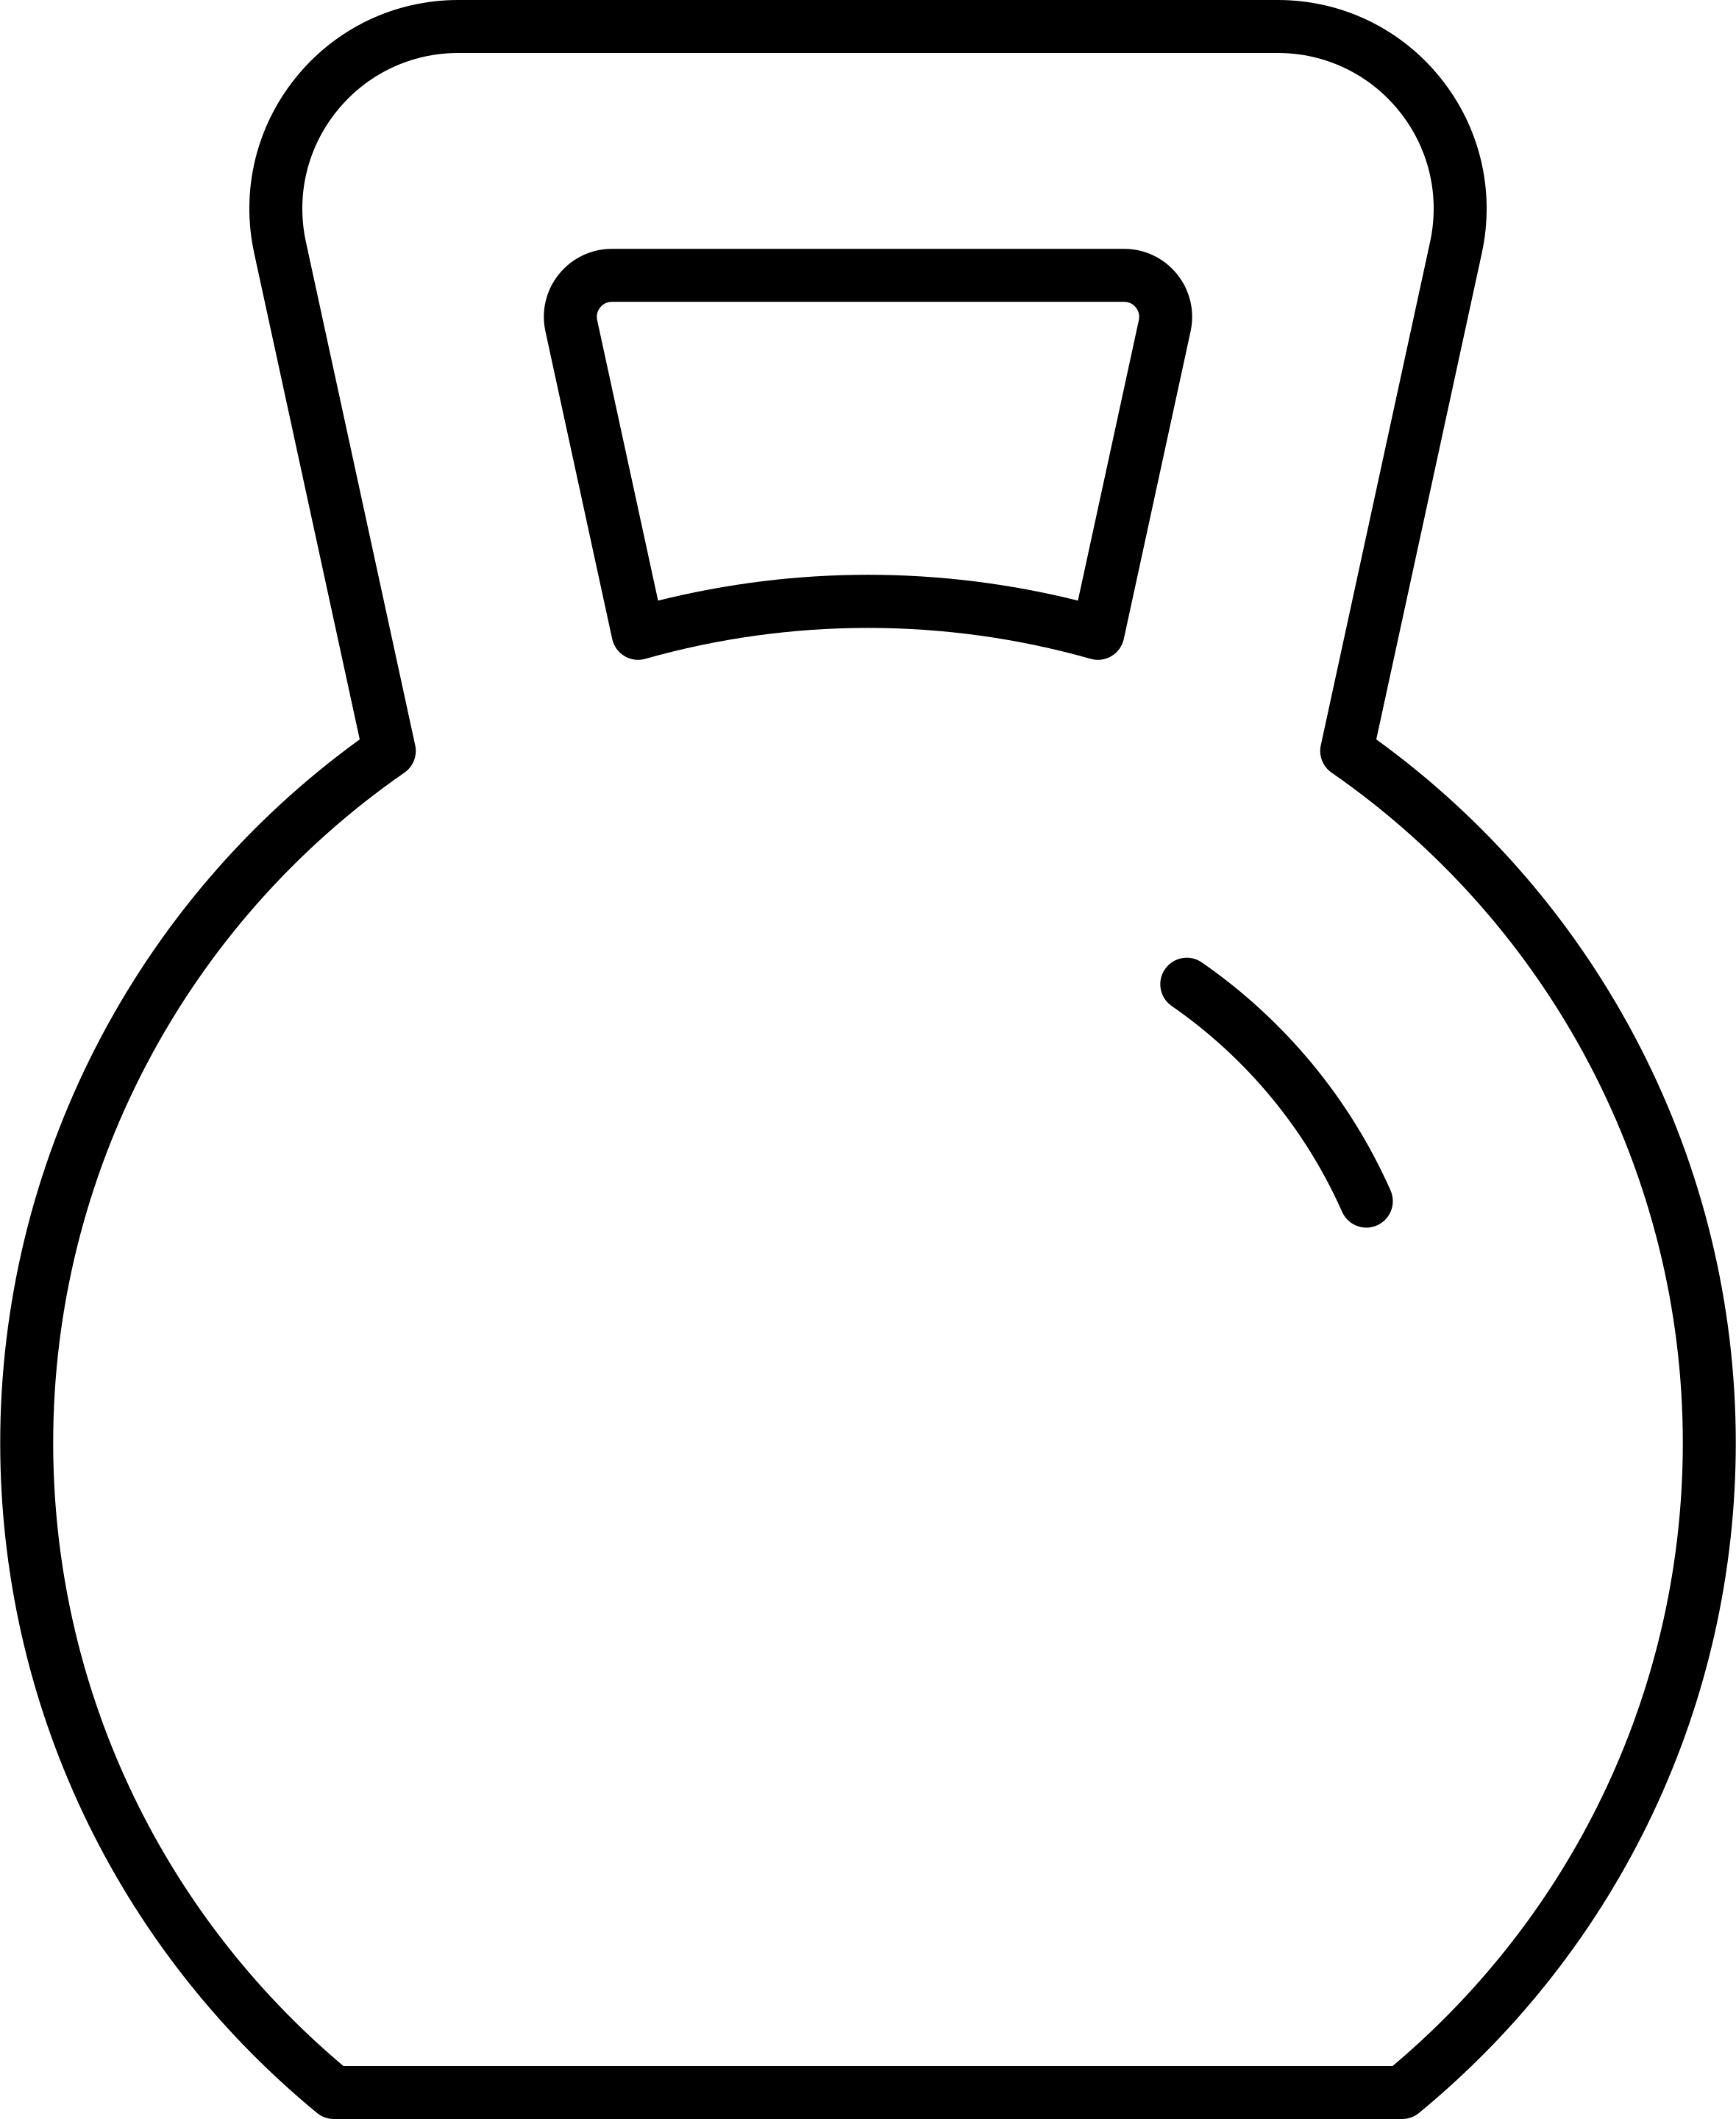
\includegraphics[width=10mm]{clipart/kettlebell}};
	\draw (\x,0)node[above,yshift=1mm]{$m_\i$};
	}
\filldraw[C3] (-1.5,-.5)--(-1.25,0)--(-1,-.5)--cycle;
\draw[C3,line width=1mm](-1.25,-.25)--(-1.25,-.75) node[below]{$\overline x$};
\end{tikzpicture}\end{center}

If the body consists of a finite number of masses $m_1$, $\cdots$, $m_n$
attached to an infinitely strong, weightless (idealized) rod with mass
number $i$ attached at position $x_i$, then the center of mass is
at the (weighted) average value of $x$:
\[
\bar x =\frac{\sum_{i=1}^n m_ix_i}{\sum_{i=1}^n m_i}
\]
The denominator $m=\sum_{i=1}^n m_i$ is the total mass of the body.

\index{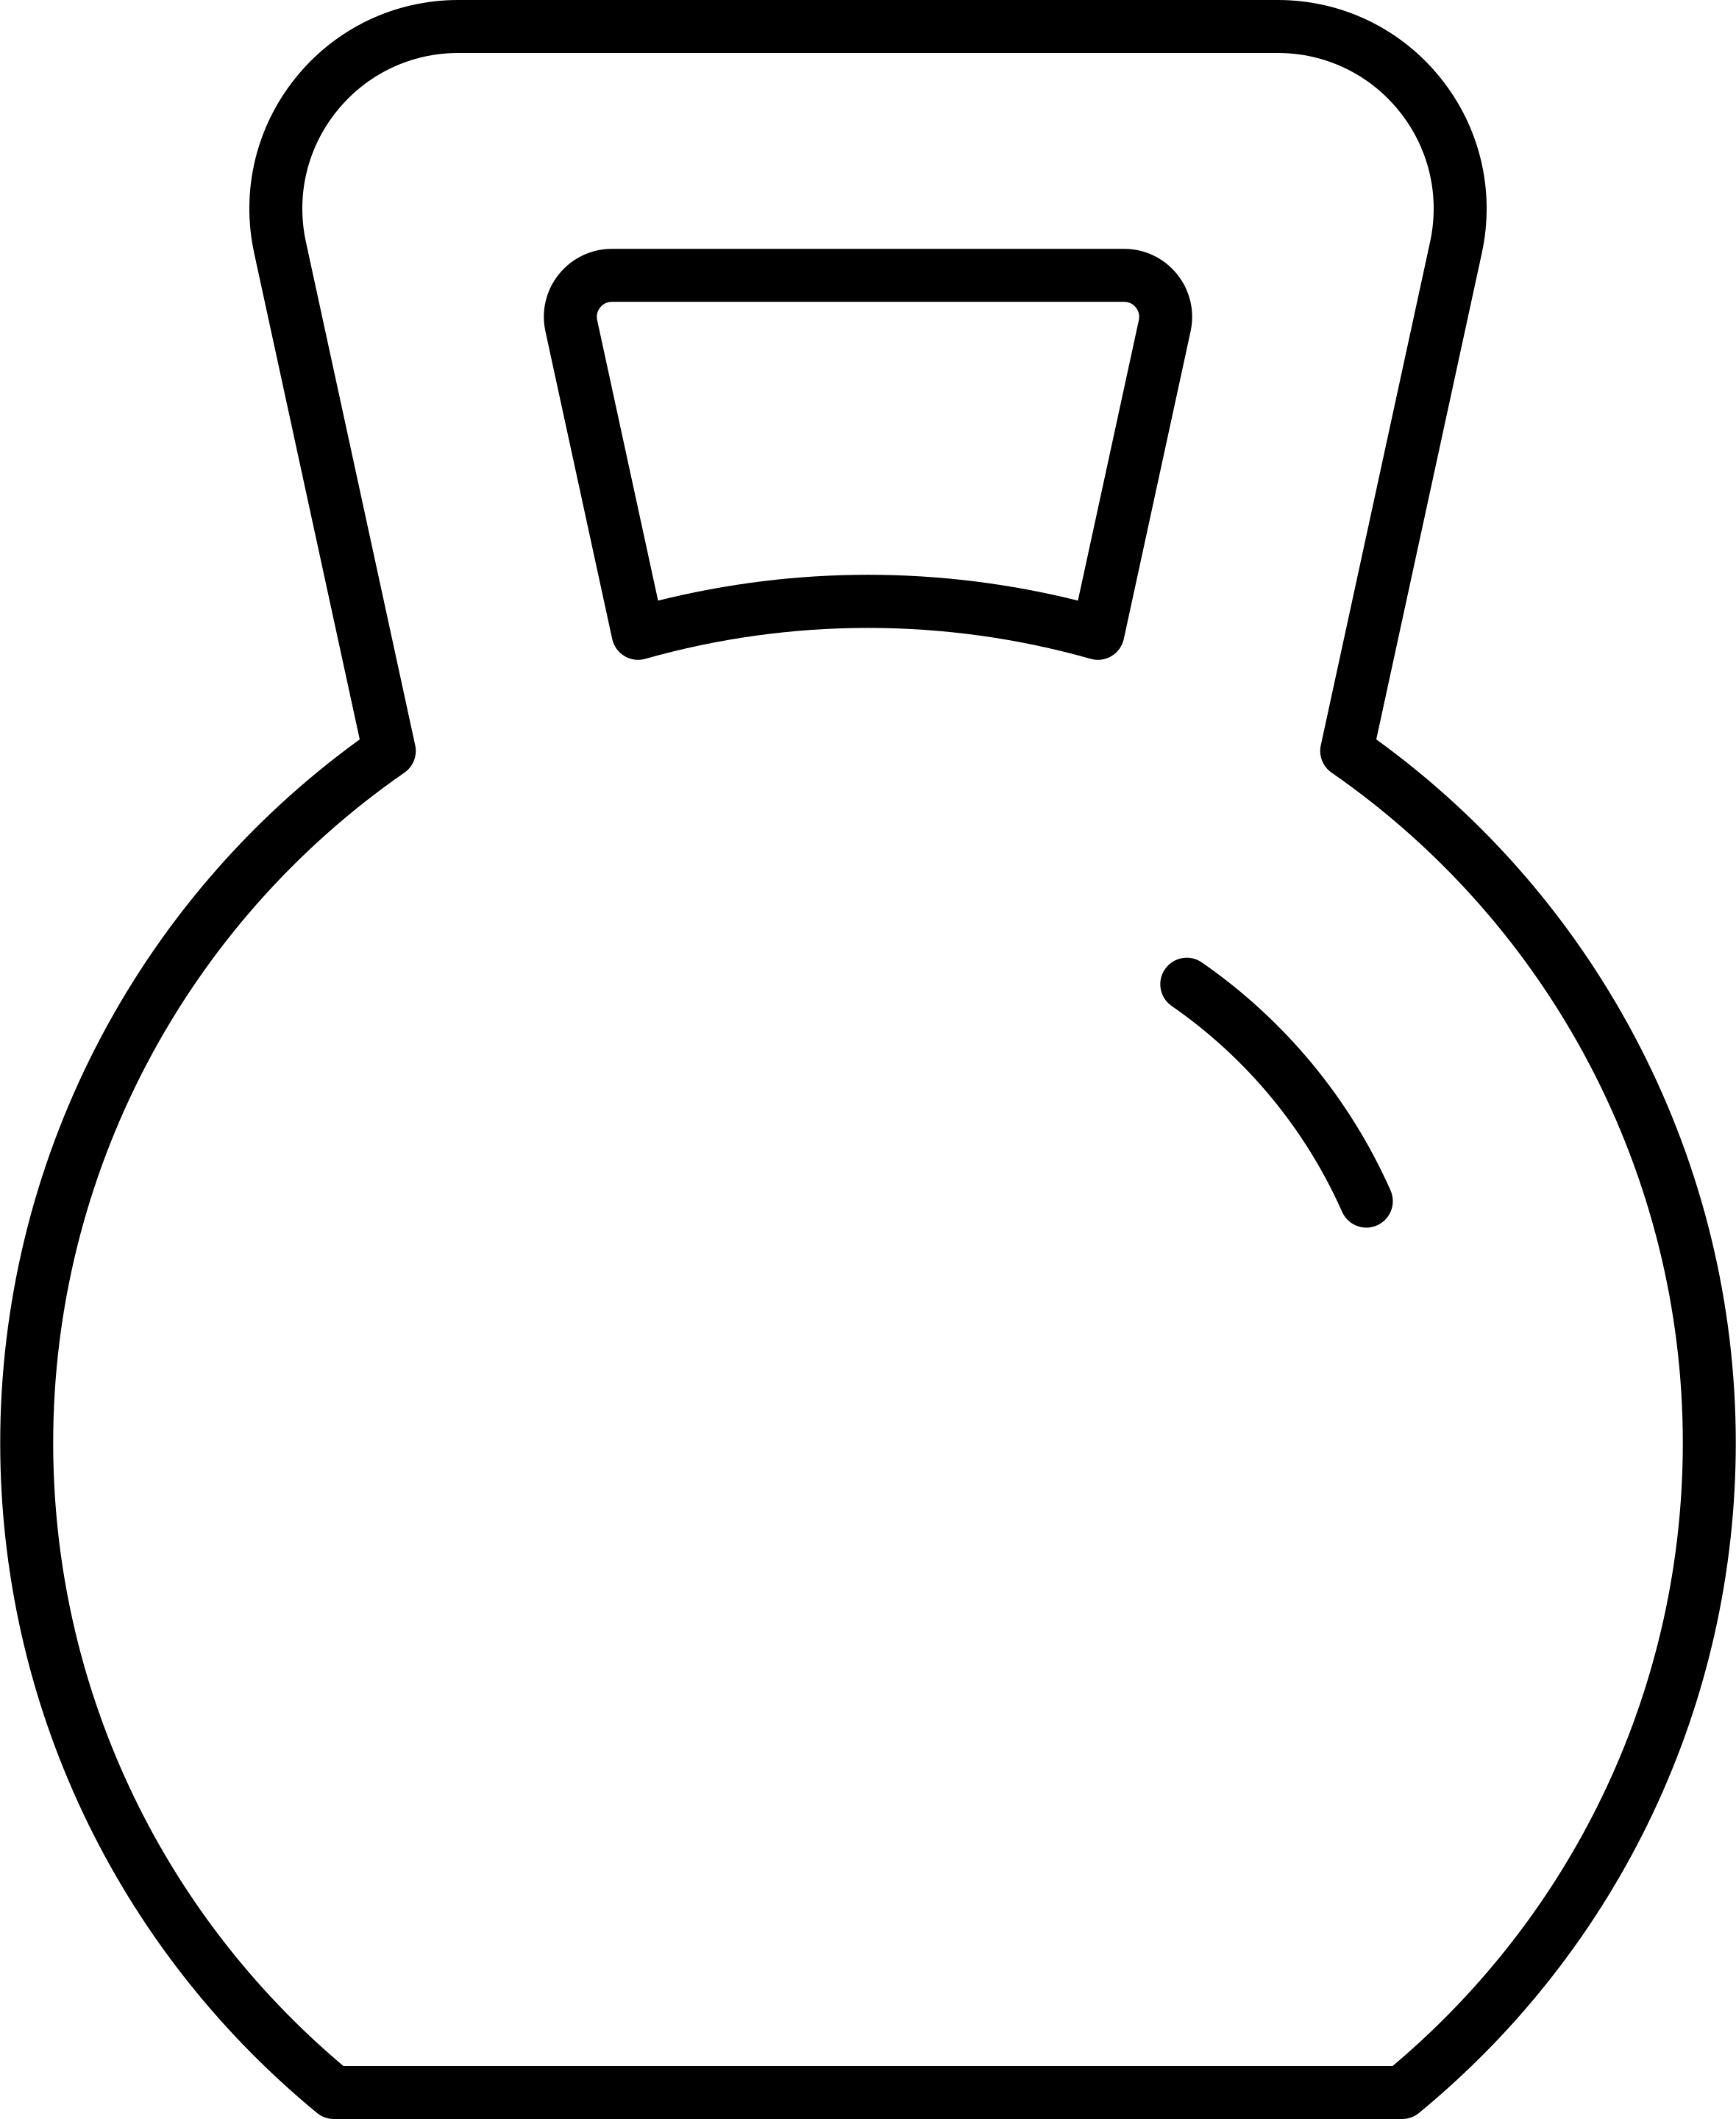
\includegraphics[height=3mm]{clipart/kettlebell} \href{https://thenounproject.com/icon/kettle-bell-3811181/}{kettle bell} by \href{https://thenounproject.com/elki/}{Made} is licensed under \CCBYthree~(accessed 10 January 2023)}

\end{frame}
%----------------------------------------------------------------------------------------
\begin{frame}[t]
\AnswerYes<1>\NoSpace<1>
An idealized (weightless, unbending) rod has small masses attached to it at the following locations:
\begin{itemize}
\item 1 kg at $x=1$ metre from the left end
\item 4 kg at $x=3$ metres from the left end
\item 2 kg at $x=6$ metres from the left end
\item 1 kg at $x=7$ metres from the left end
\end{itemize}

\begin{center}
\begin{tikzpicture}
\draw (0,0)--(8,0);
\foreach \x/\i in {1/1,3/4,6/2,7/1}{
	\draw(\x,0)--(\x,-.2)node[below]{$\x$};
	\draw (\x,0)node[above, inner sep=0]{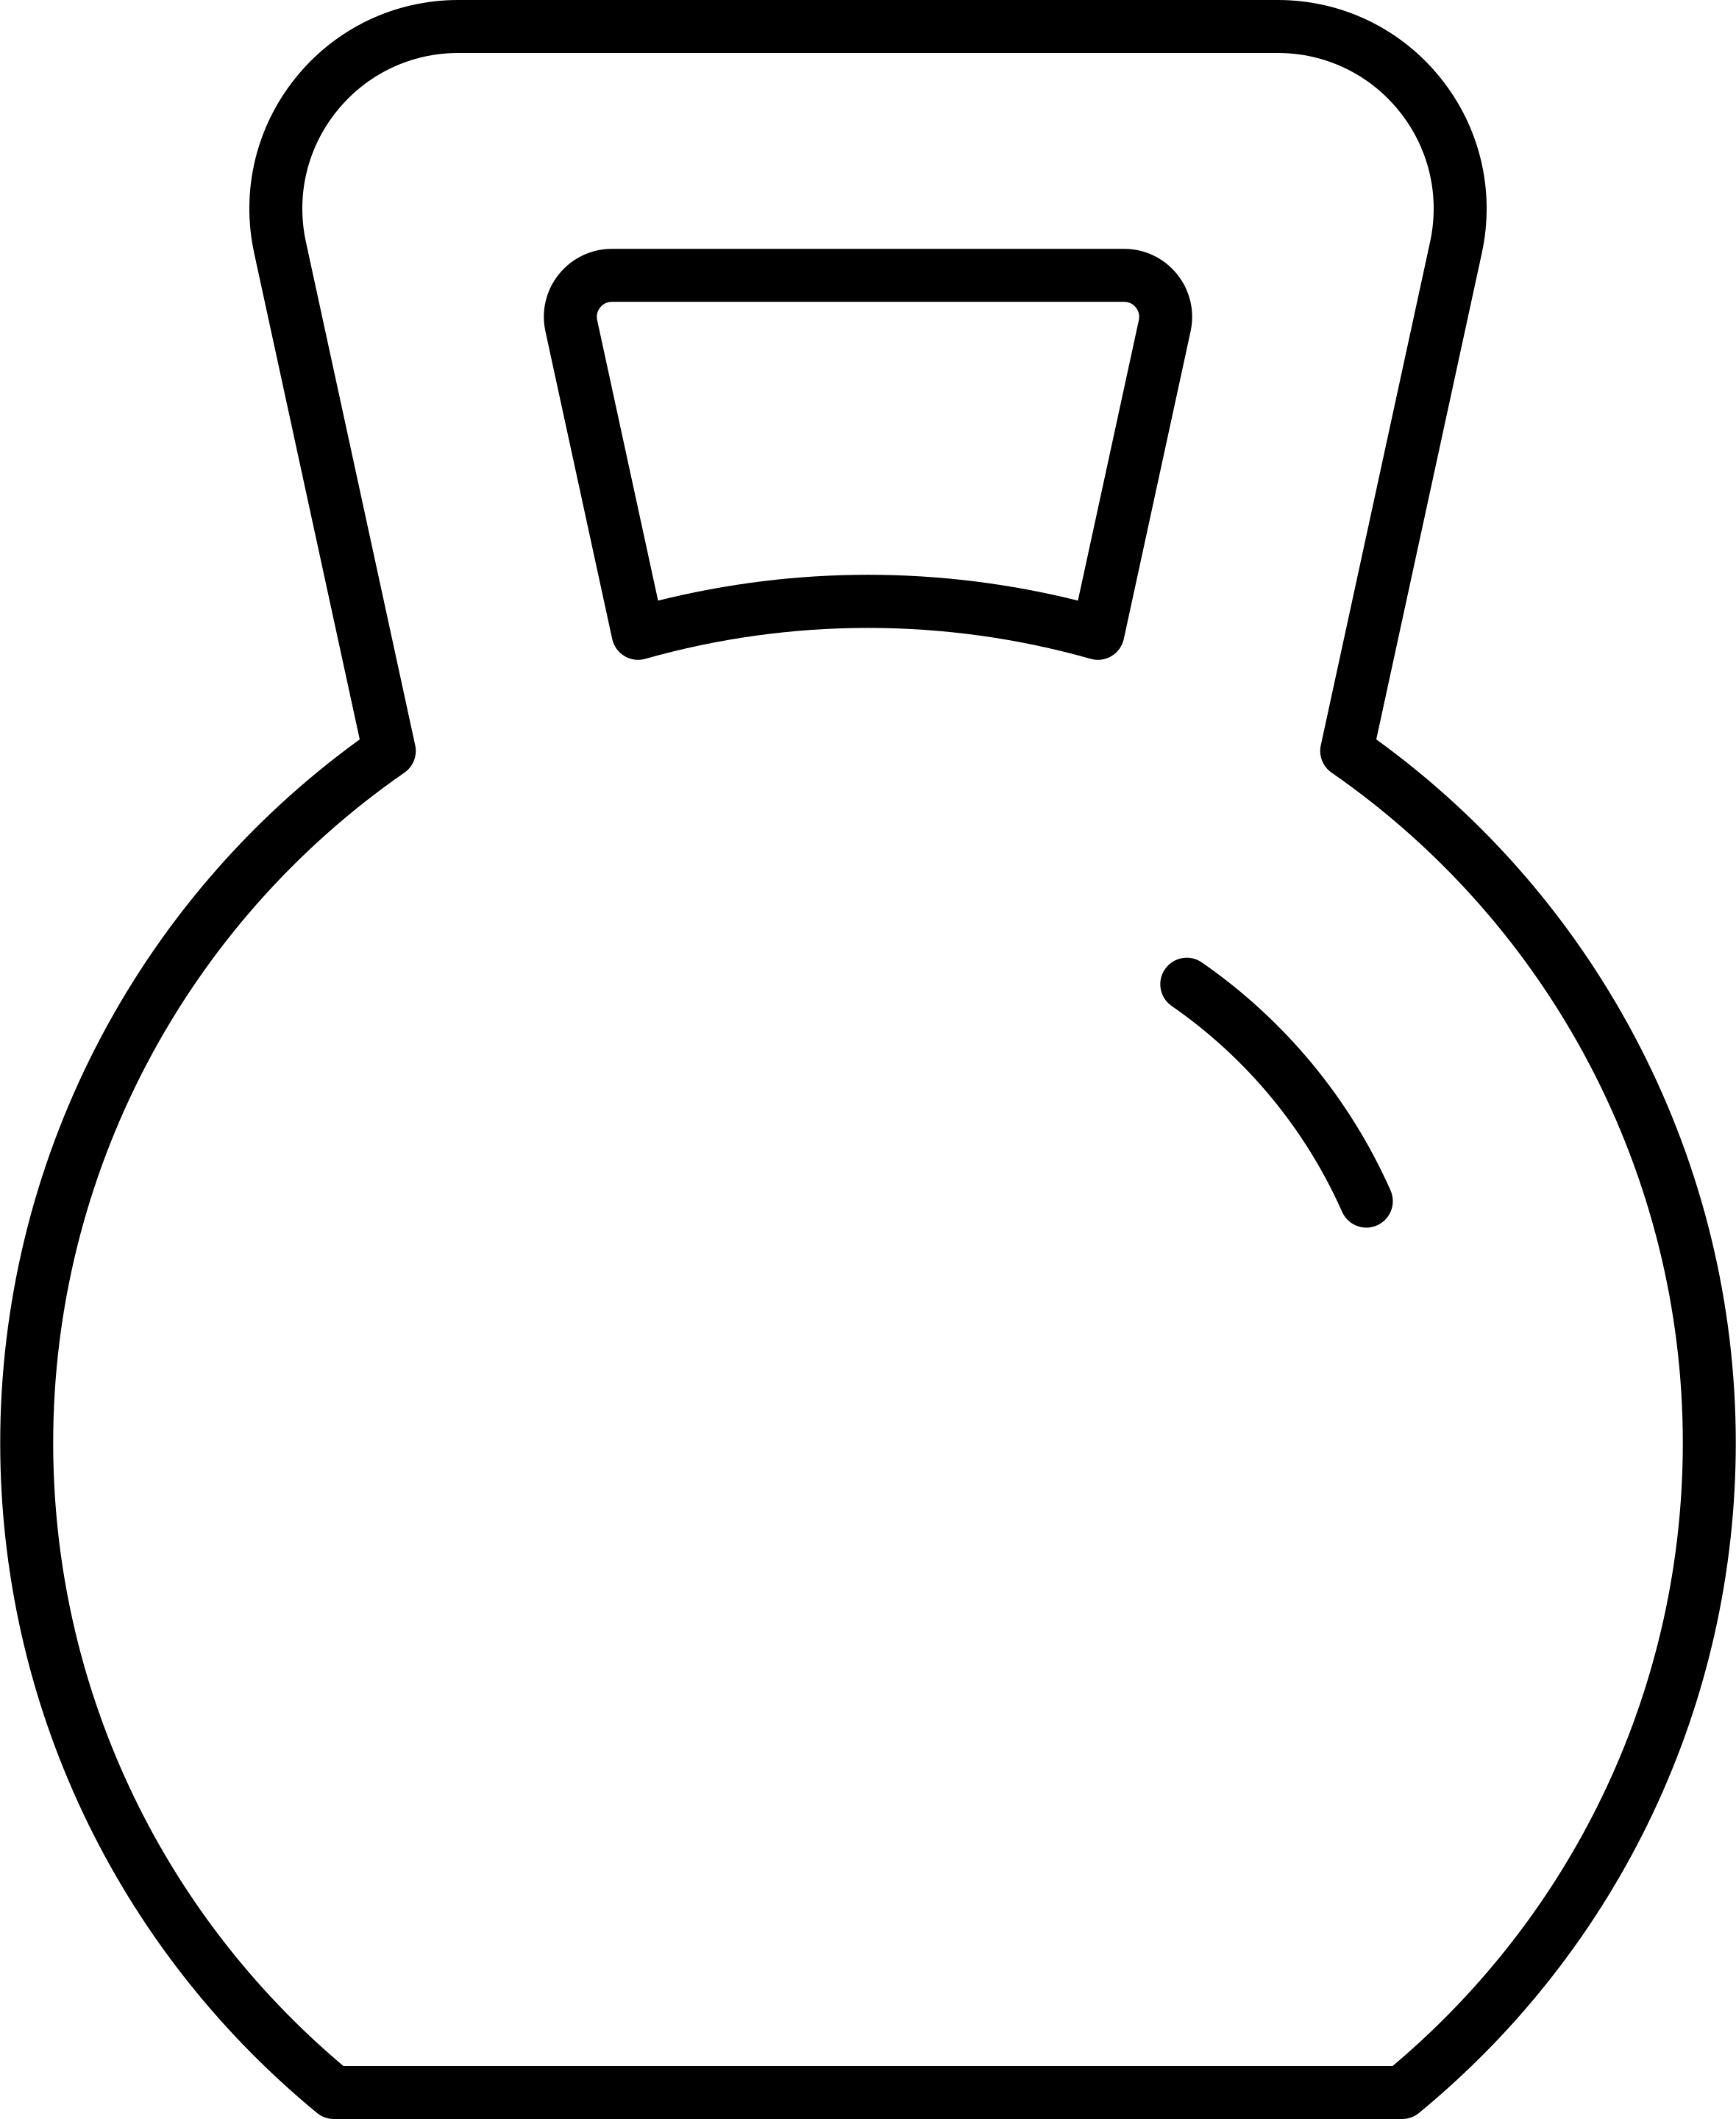
\includegraphics[width=10mm]{clipart/kettlebell}};
	\draw (\x,0)node[above]{$\i$ kg};
	}
\sonslide<2->{\fill[C3] (3.8,-.5)--(4,0)--(4.2,-.5)--cycle;}
\end{tikzpicture}
\end{center}
What is the location of its centre of mass?

\sonslide<2->{
	\[\bar x =\frac{\sum_{i=1}^n m_ix_i}{\sum_{i=1}^n m_i}
	=
	\frac{1(1)+4(3)+2(6)+1(7)}{1+4+2+1}=4\]
	So the centre of mass is 4 metres from the left end of the rod.
		}


\index{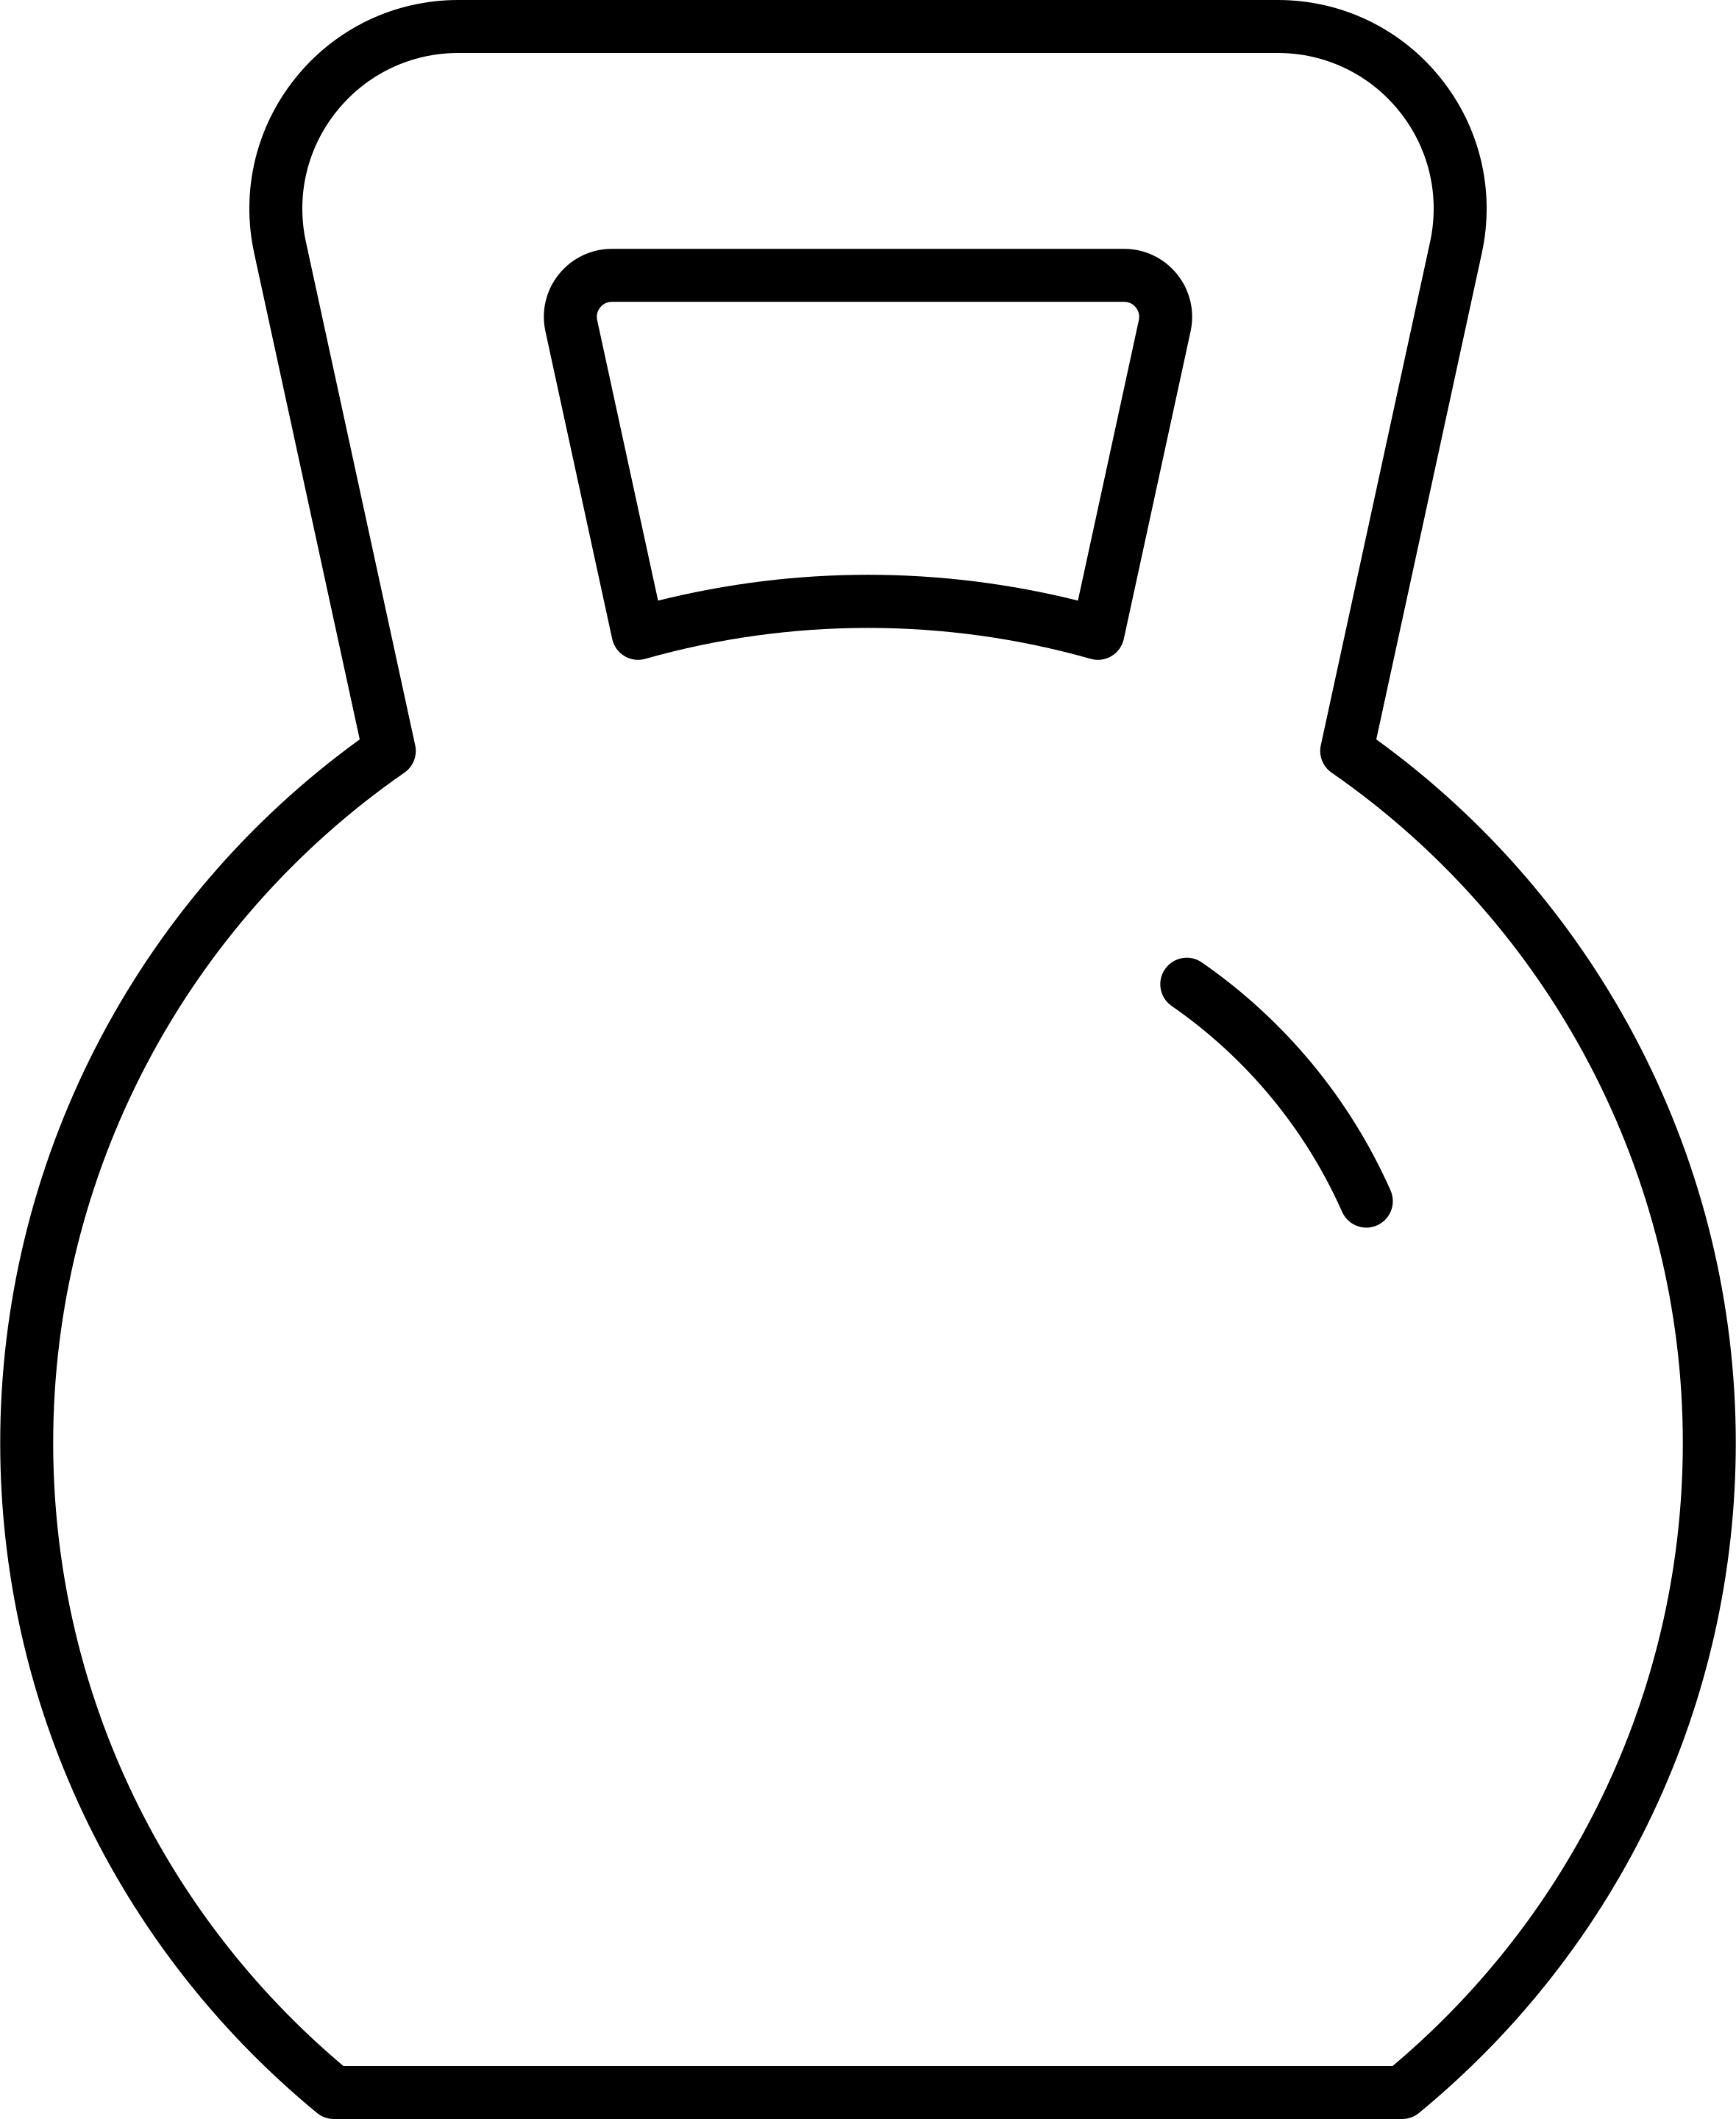
\includegraphics[height=3mm]{clipart/kettlebell} \href{https://thenounproject.com/icon/kettle-bell-3811181/}{kettle bell} by \href{https://thenounproject.com/elki/}{Made} is licensed under \CCBYthree~(accessed 10 January 2023)}

\end{frame}
%----------------------------------------------------------------------------------------
\begin{frame}[t]
\sStatusBar{1}{4}
\MoreSpace<1>
\AnswerYes<1-3>
\only<1>{We can also group the masses, and treat them as single points of mass at their centres of gravity, without affecting the centre of gravity of the entire object.}
\begin{center}
\begin{tikzpicture}
\draw (0,0)--(8,0);
\foreach \x/\i in {1/1,3/4,6/2,7/1}{
	\draw(\x,0)--(\x,-.2)node[below]{$\x$};
	\draw (\x,0)node[above, inner sep=0]{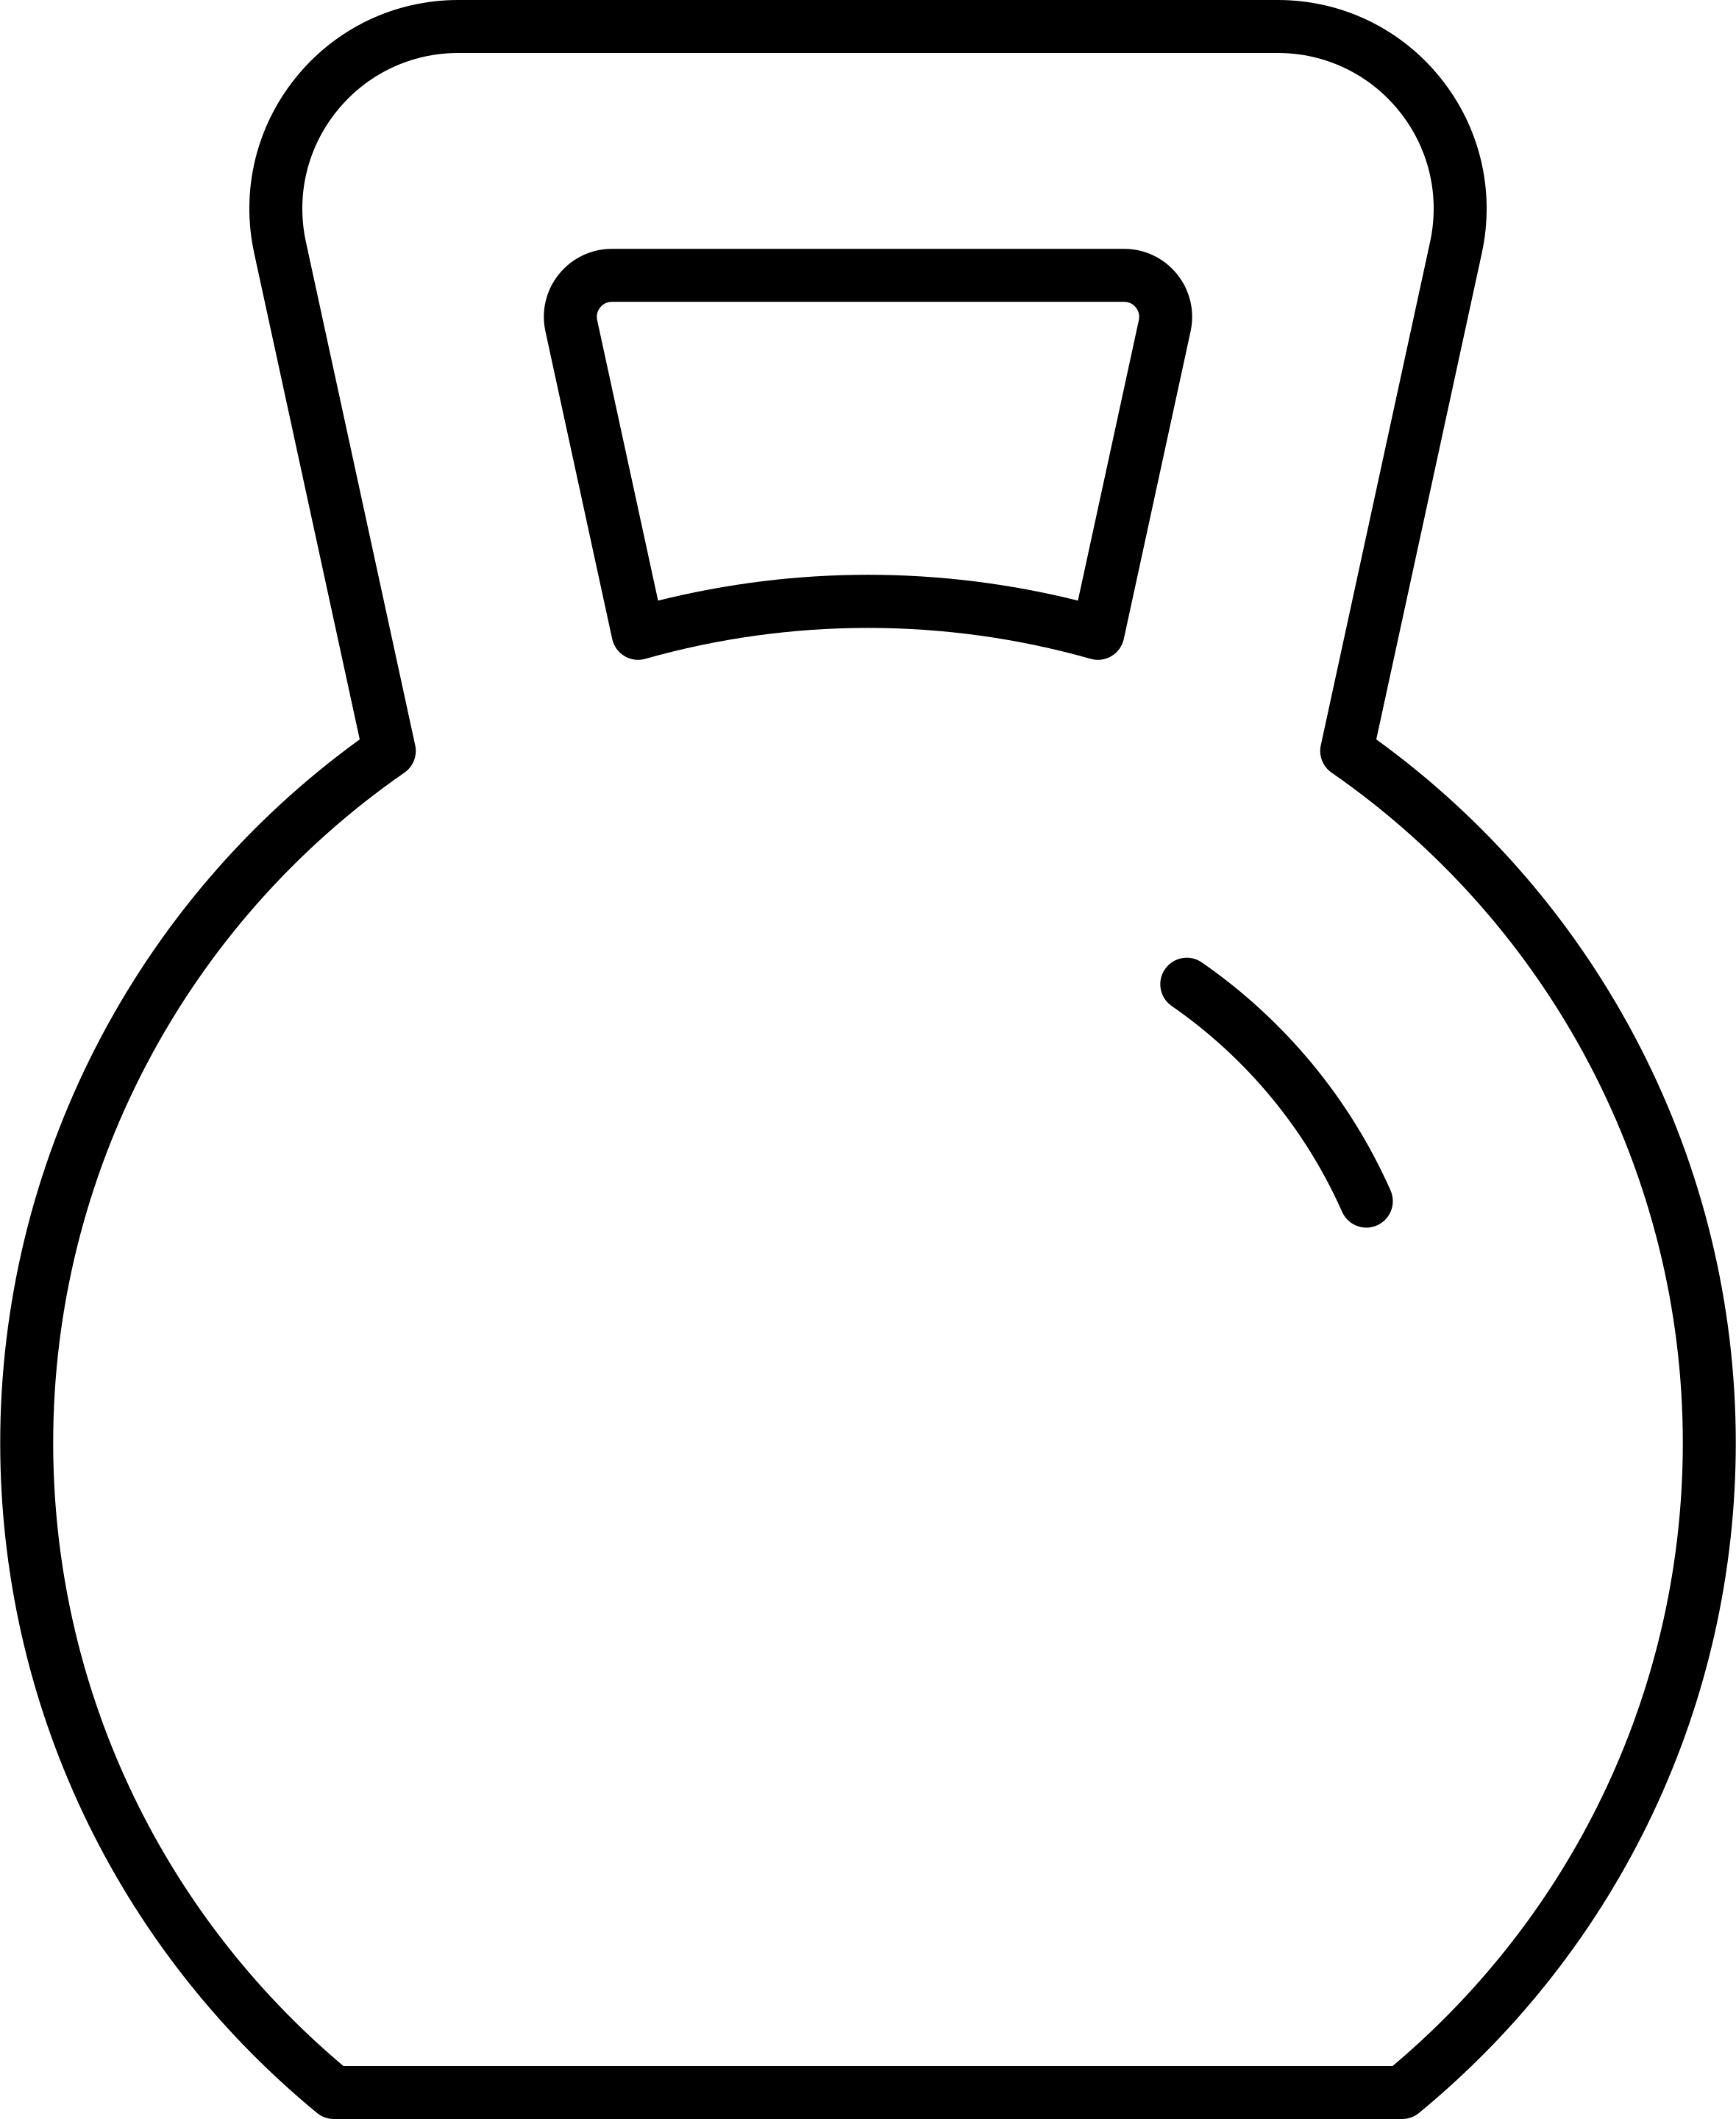
\includegraphics[width=10mm]{clipart/kettlebell}};
	\draw (\x,0)node[above]{$\i$ kg};
	}
\draw[W1,decorate,decoration={brace,mirror,amplitude=3mm}] (0,-.6)--(4,-.6)node[midway,below,yshift=-3mm]{Centre of mass:};
\sonslide<2->{\draw (2,-1.75)node[W1]{$\frac{1(1)+4(3)}{1+4}=\frac{13}{5}$};}

\draw[C1,decorate,decoration={brace,mirror,amplitude=3mm}] (5,-.6)--(8,-.6)node[midway,below,yshift=-3mm]{Centre of mass:};
\sonslide<2->{\draw (6.5,-1.75)node[C1]{$\frac{2(6)+1(7)}{2+1}=\frac{19}{3}$};}
\end{tikzpicture}

%second rod
\vfill\begin{tikzpicture}
\onslide<3->{
	\draw (0,0)--(8,0);
	{\color{W1}

	\draw (2.6,0)node[above, inner sep=0]{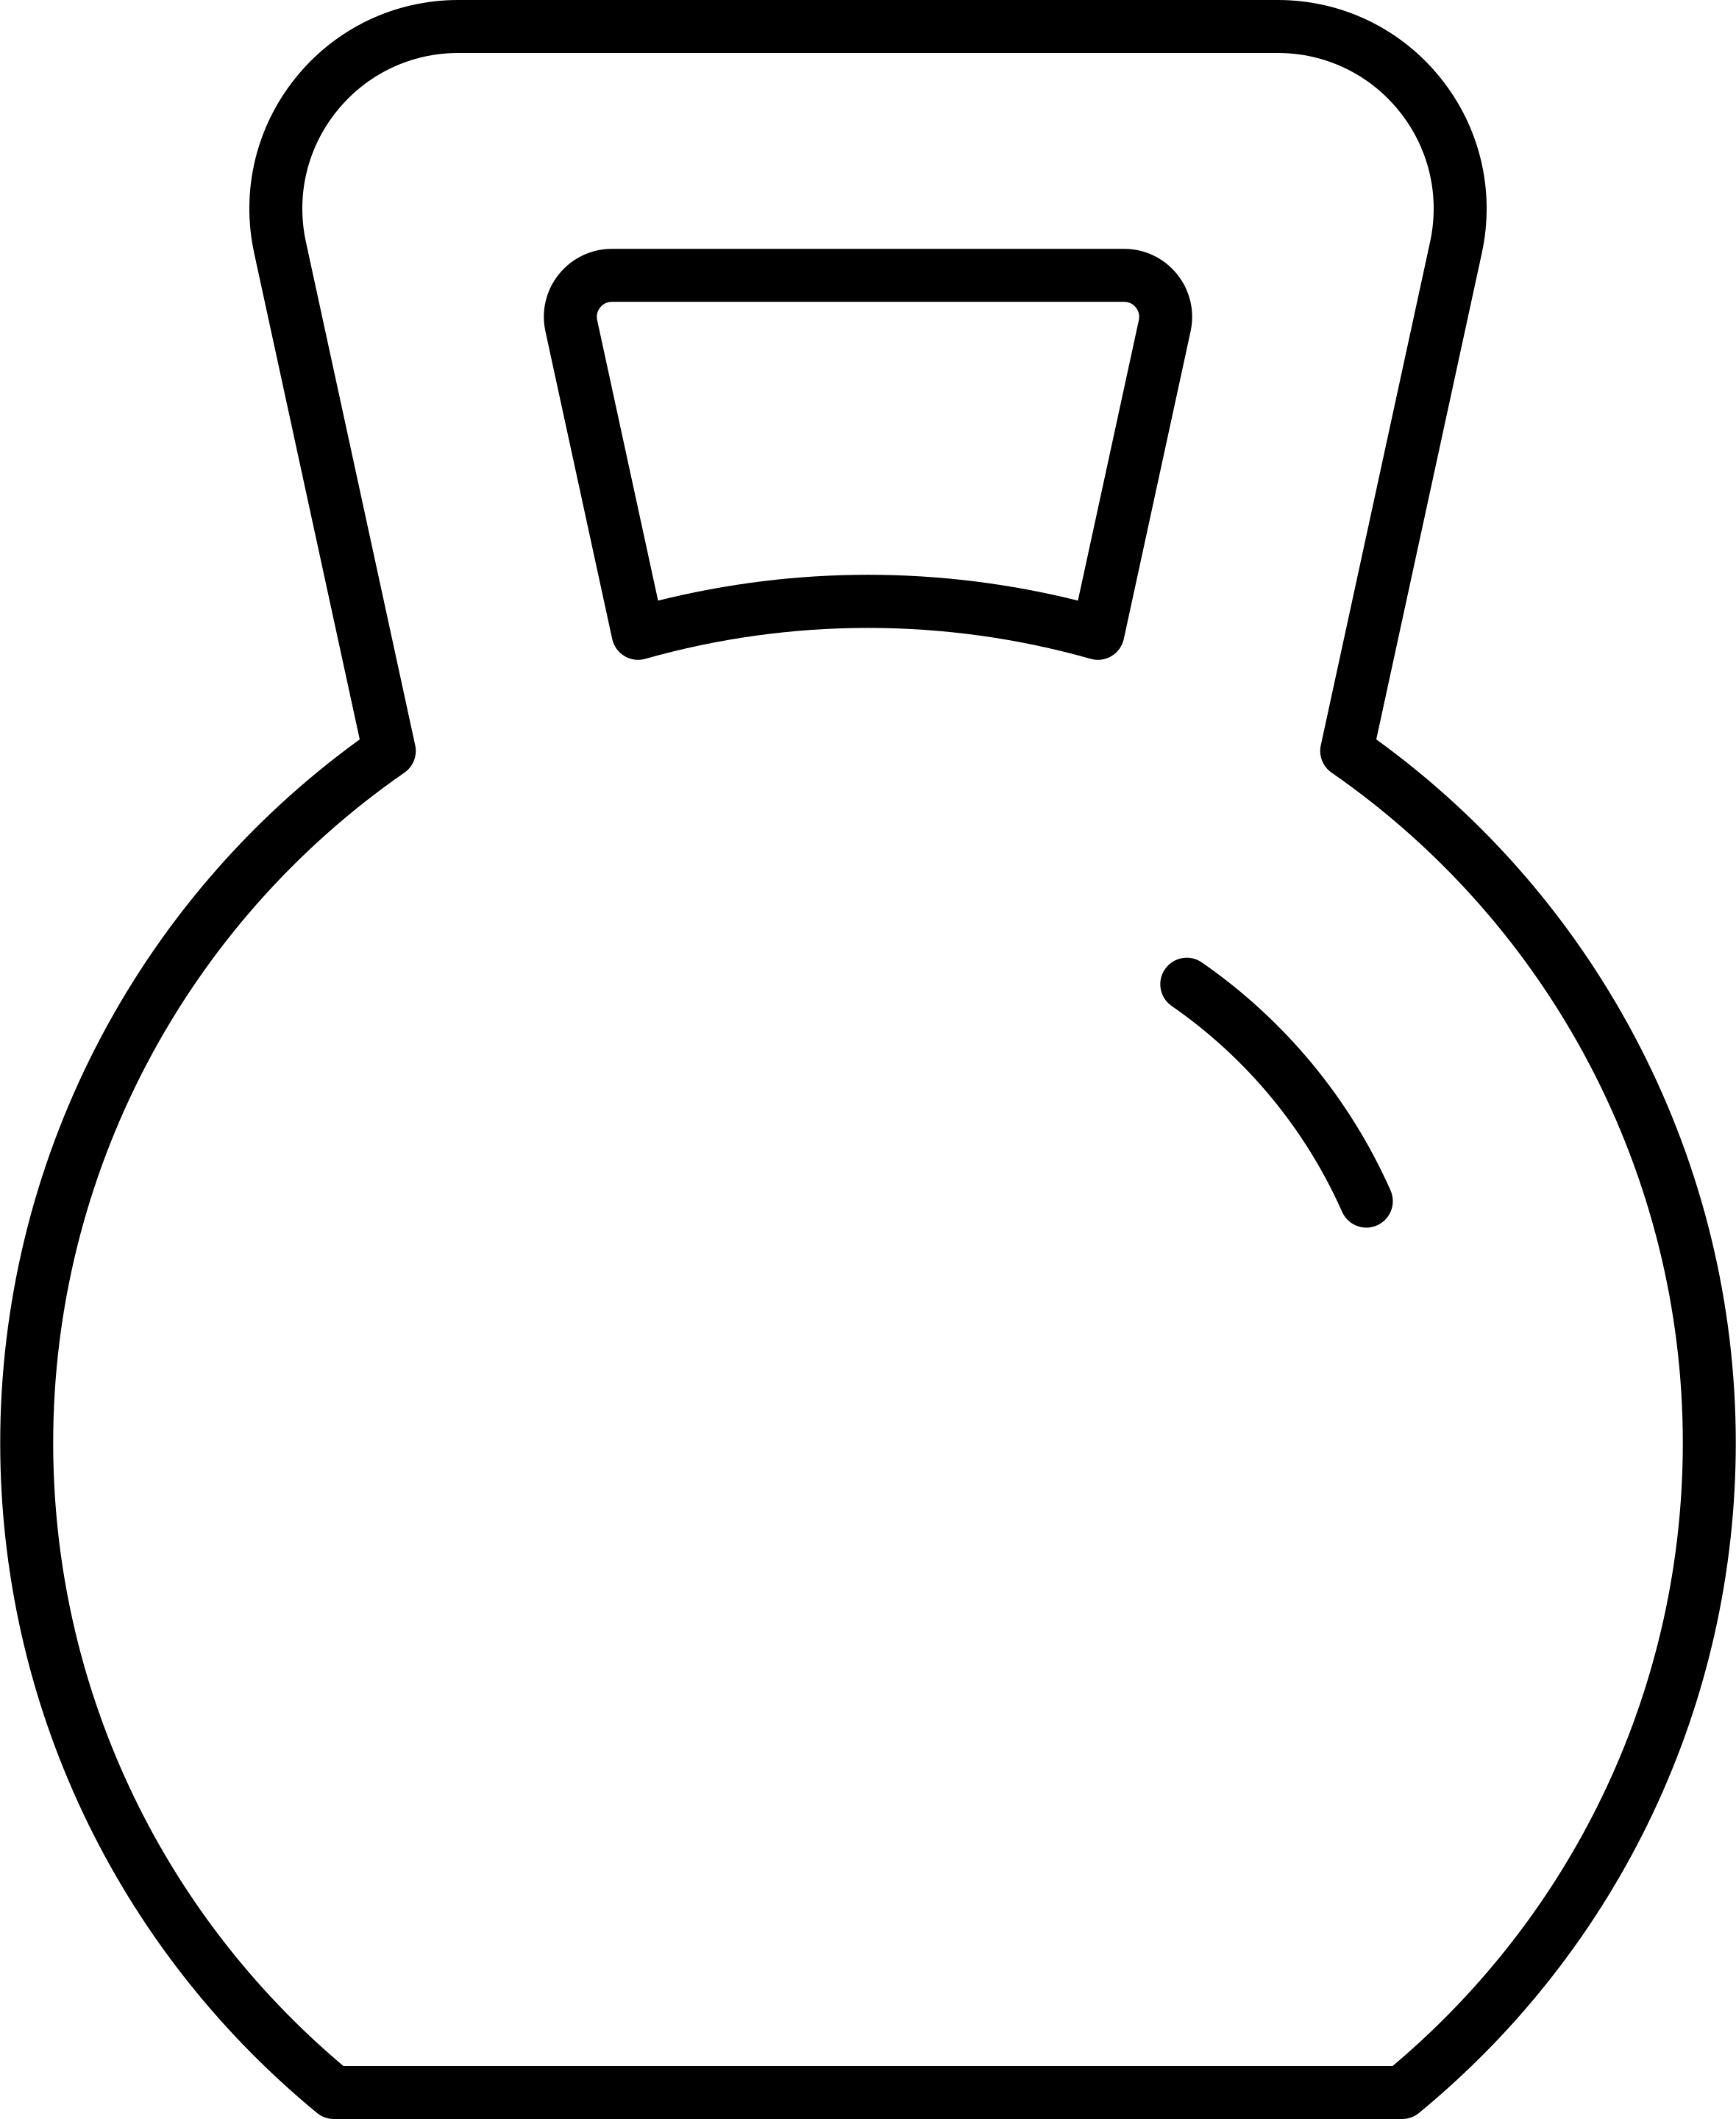
\includegraphics[width=10mm]{clipart/kettlebell}};
	\only<beamer>{\draw(2.6,0)--(2.6,-.2)node[below]{$\frac{13}{5}$};
		\draw (2.6,0)node[above]{$5$ kg};}}
	{\color{C1}
	\draw (6.33,0)node[above, inner sep=0]{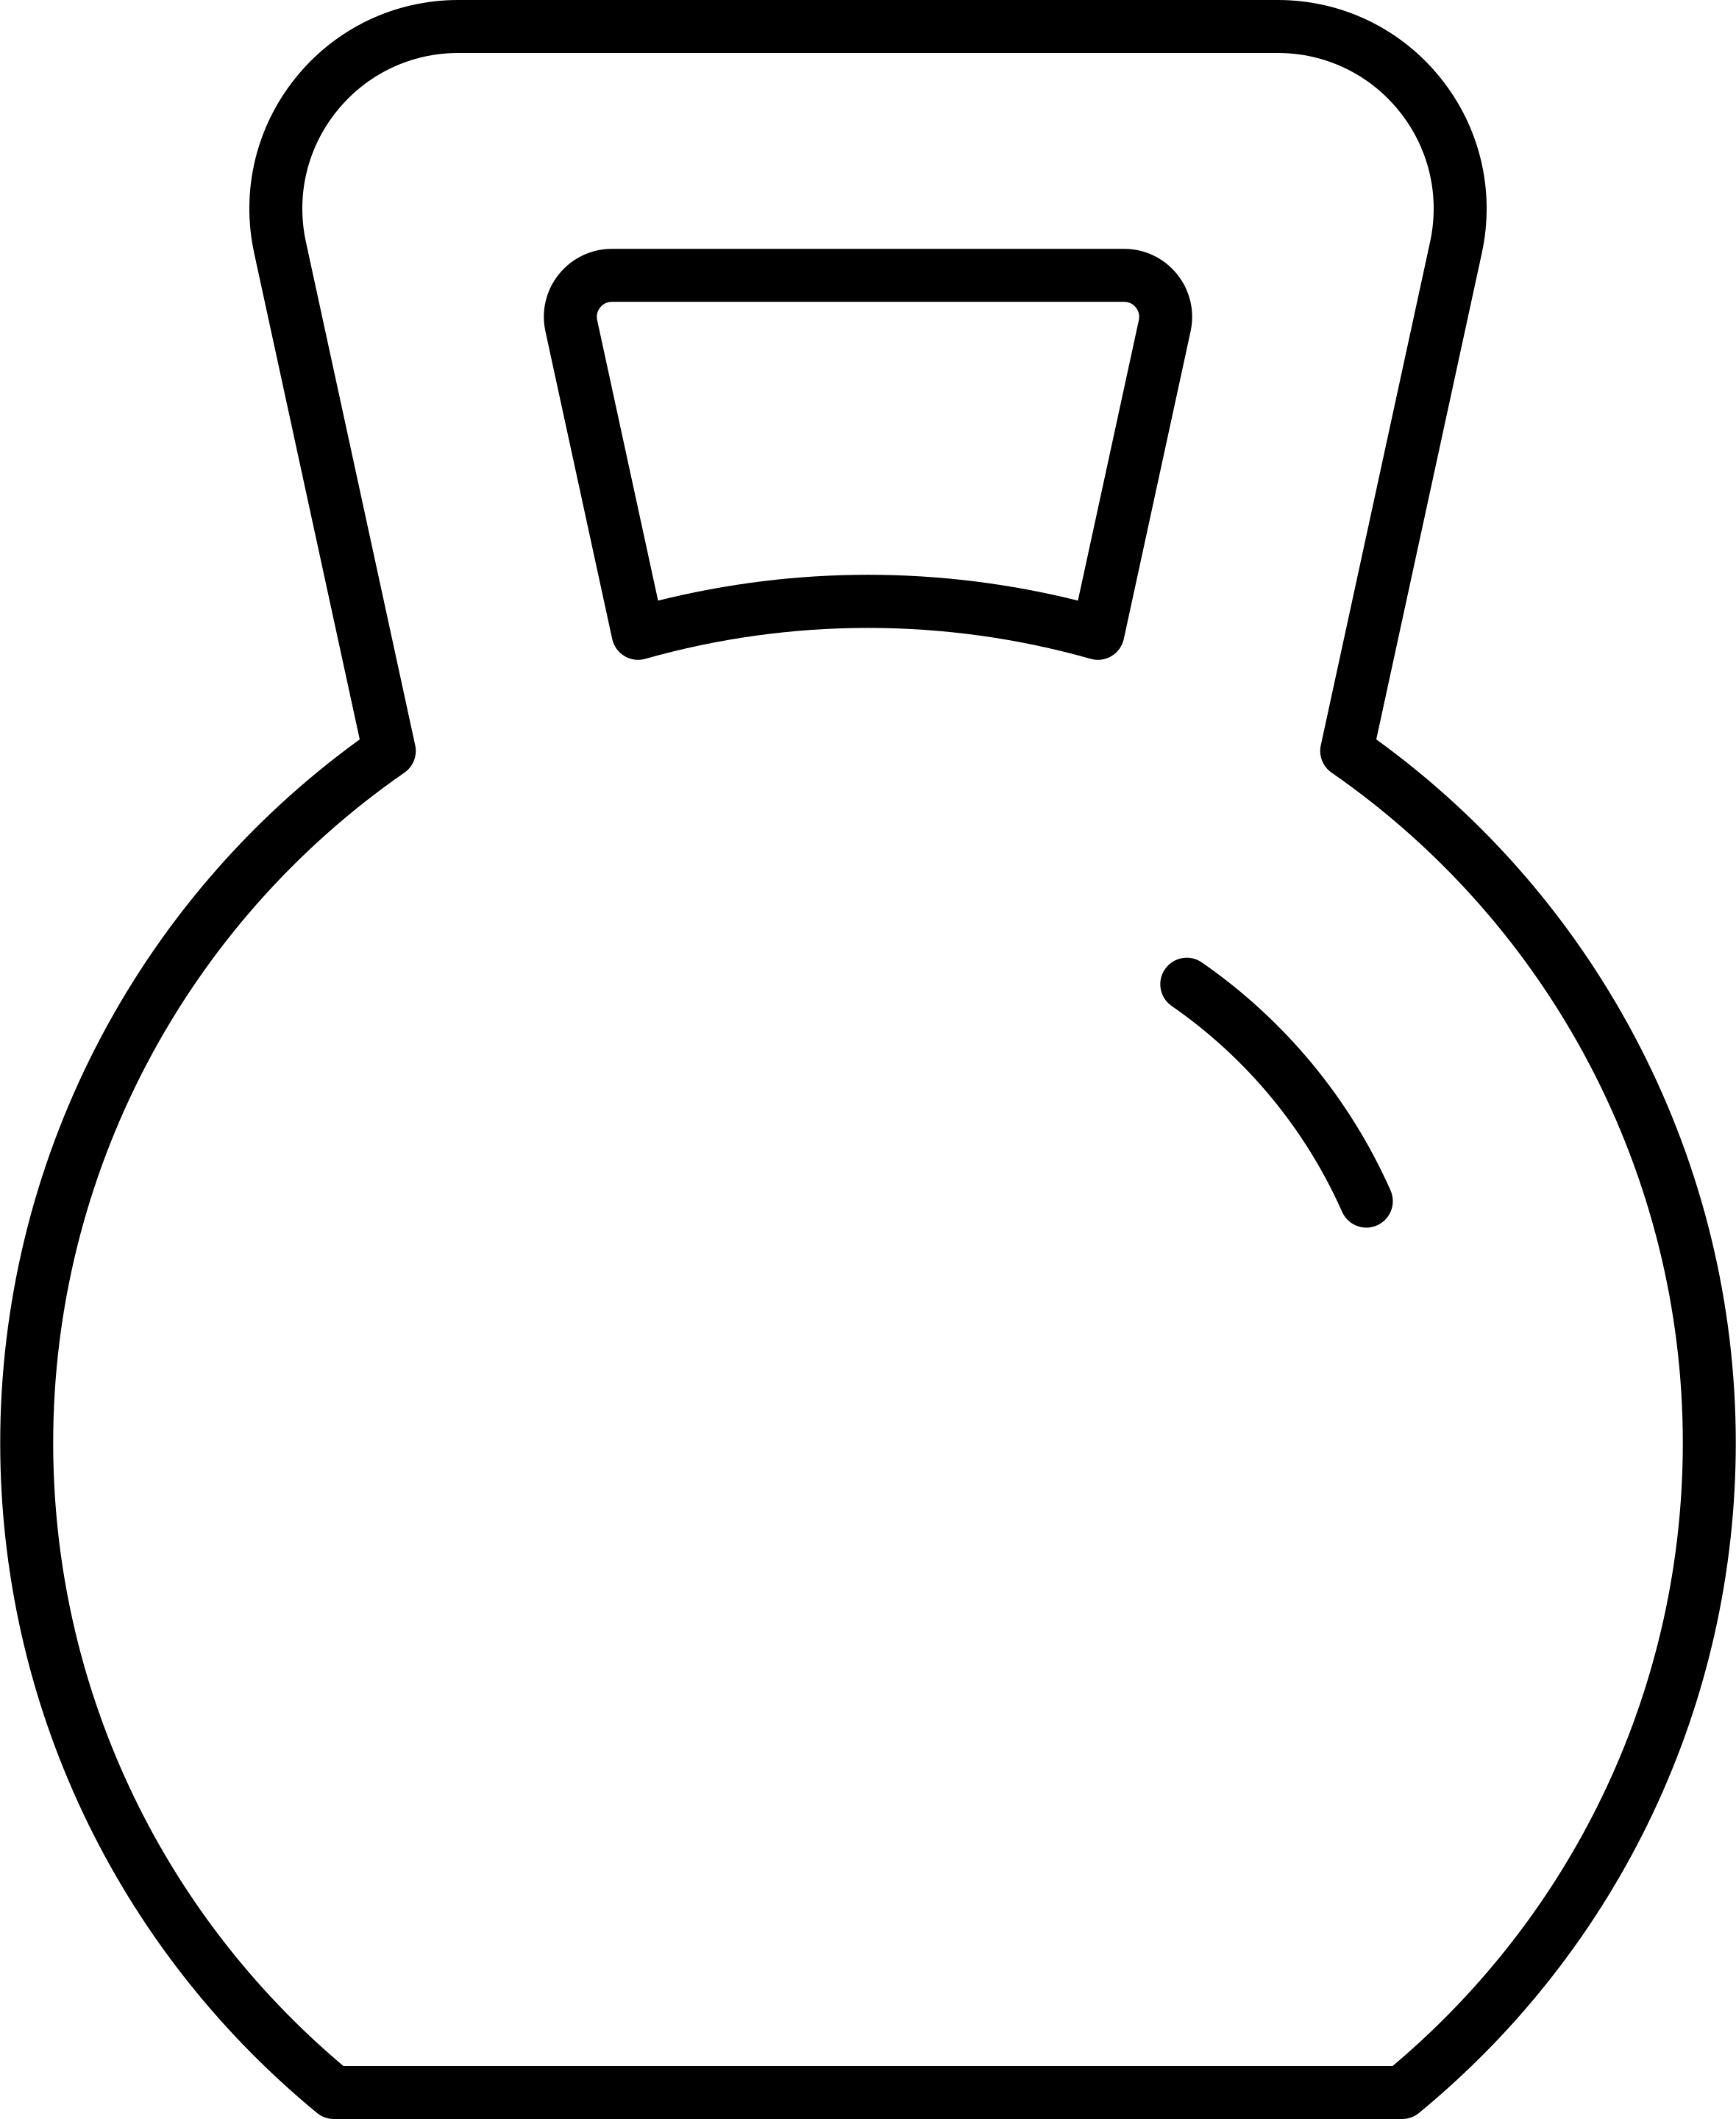
\includegraphics[width=10mm]{clipart/kettlebell}};
	\only<beamer>{\draw(6.33,0)--(6.33,-.2)node[below]{$\frac{19}{3}$};
	\draw (6.33,0)node[above]{$3$ kg};}}
	}
\end{tikzpicture}
\end{center}
\vfill
\sonslide<4->{Centre of mass of second rod: $\bar x=\frac{5\left(\frac{13}{5}\right)+3\left(\frac{19}{3}\right)}{5+3}=4$}


\index{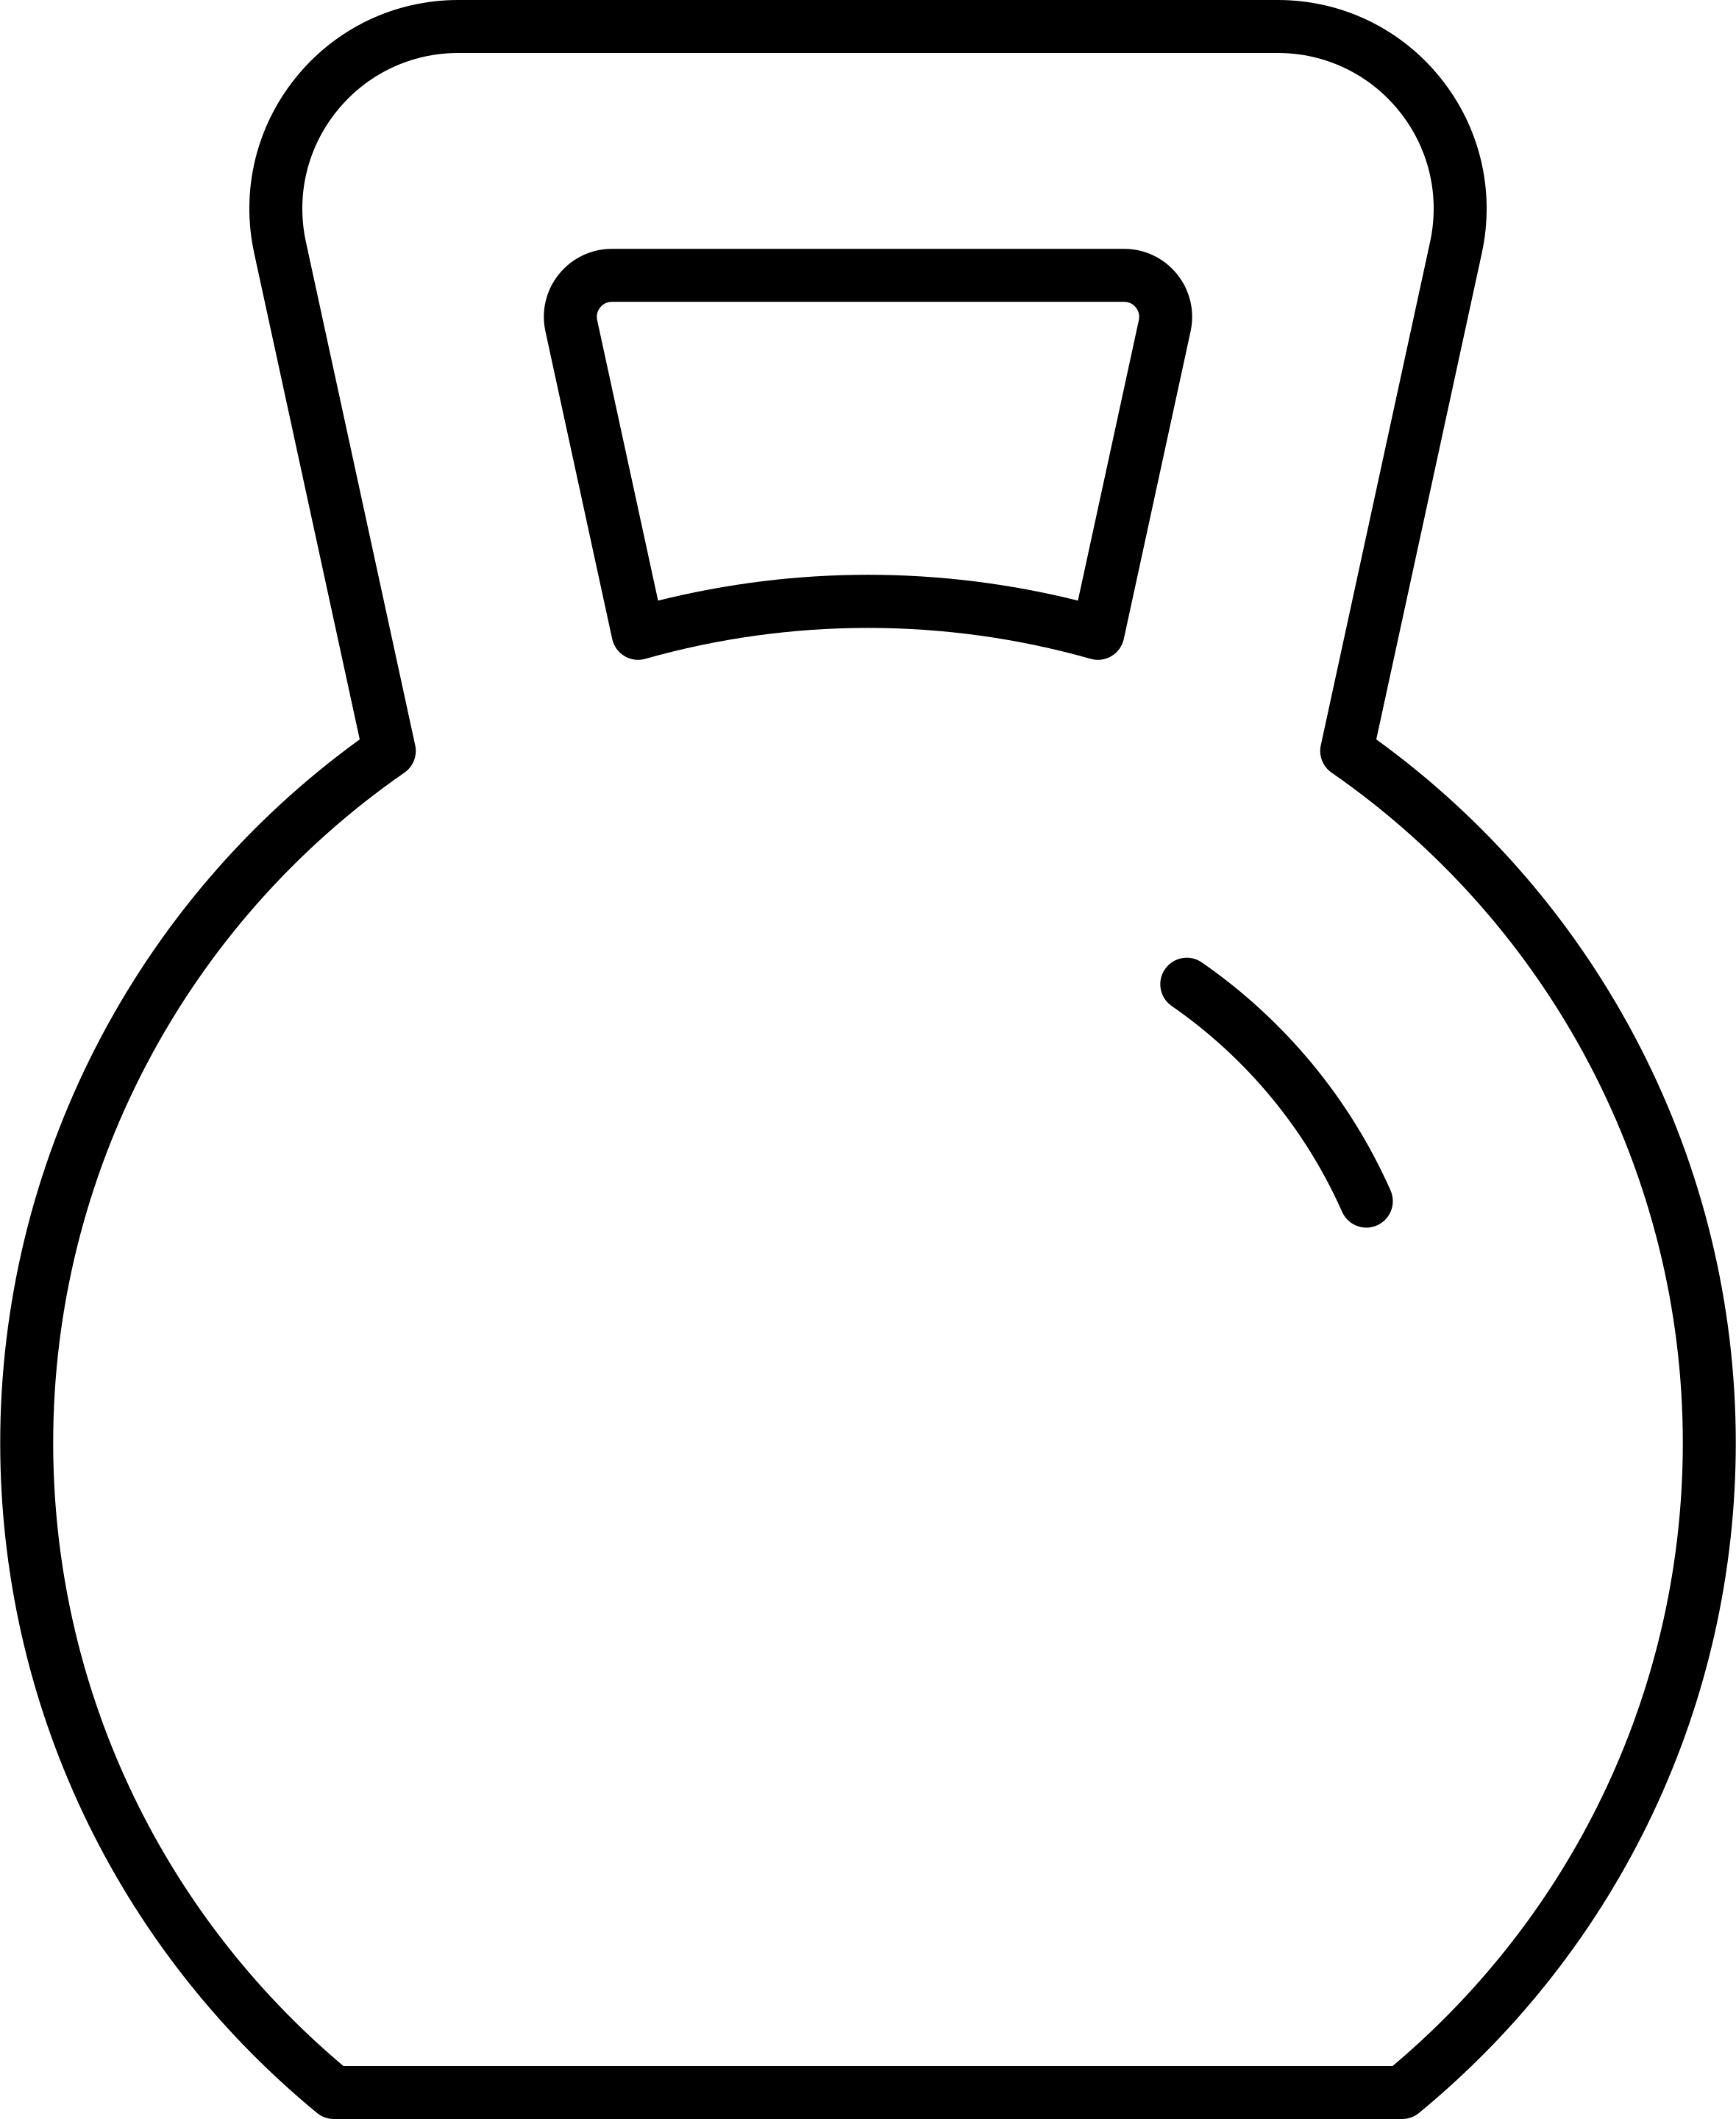
\includegraphics[height=3mm]{clipart/kettlebell} \href{https://thenounproject.com/icon/kettle-bell-3811181/}{kettle bell} by \href{https://thenounproject.com/elki/}{Made} is licensed under \CCBYthree~(accessed 10 January 2023)}

\end{frame}
%----------------------------------------------------------------------------------------
\begin{frame}[t]
\MoreSpace<1>
\AnswerYes<2>
Sometimes we can simplify a physical calculation by treating an object as a point particle located at its centre of mass.

When we were learning about work, we found the following:

\begin{multicols}{2}
\only<1>{\index{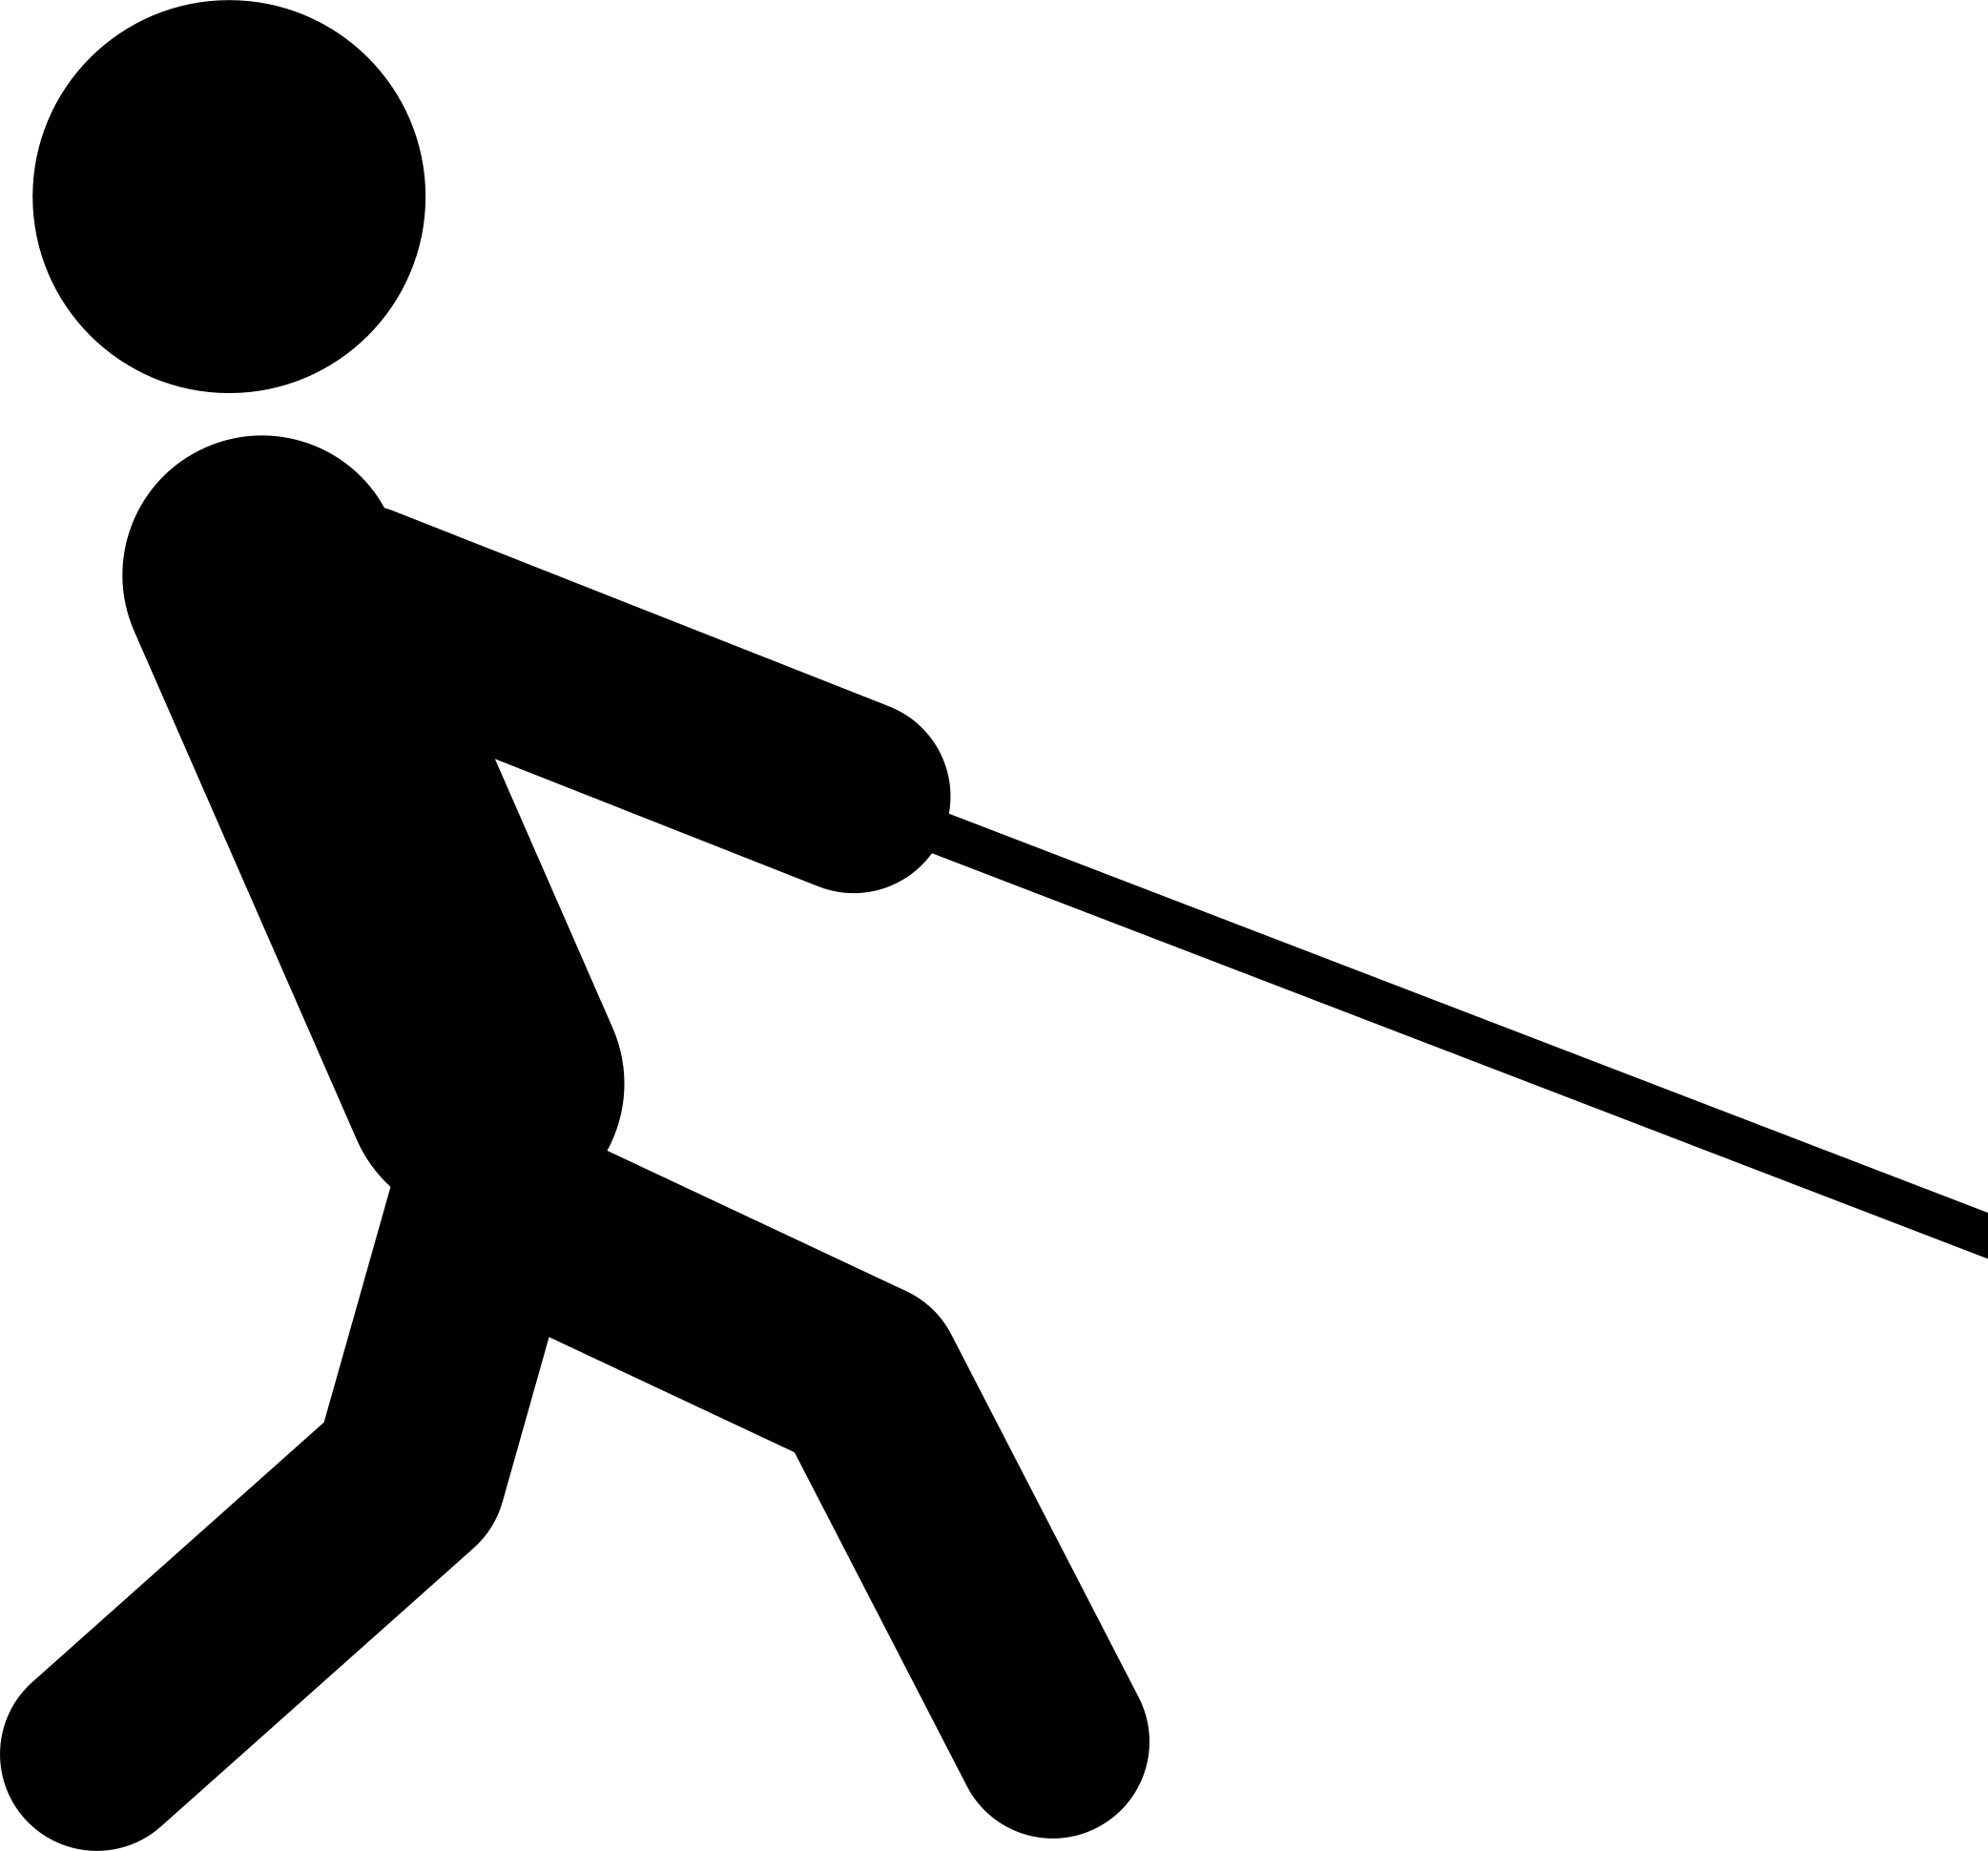
\includegraphics[height=3mm]{clipart/pull} \href{https://thenounproject.com/icon/pull-23535/}{pull}  by \href{https://thenounproject.com/pavel.nikandrov/}{Pavel N} is licensed under \CCBYthree~(accessed 10 January 2023, modified)}

\begin{tikzpicture}
\draw(0,-0.005)node[left]{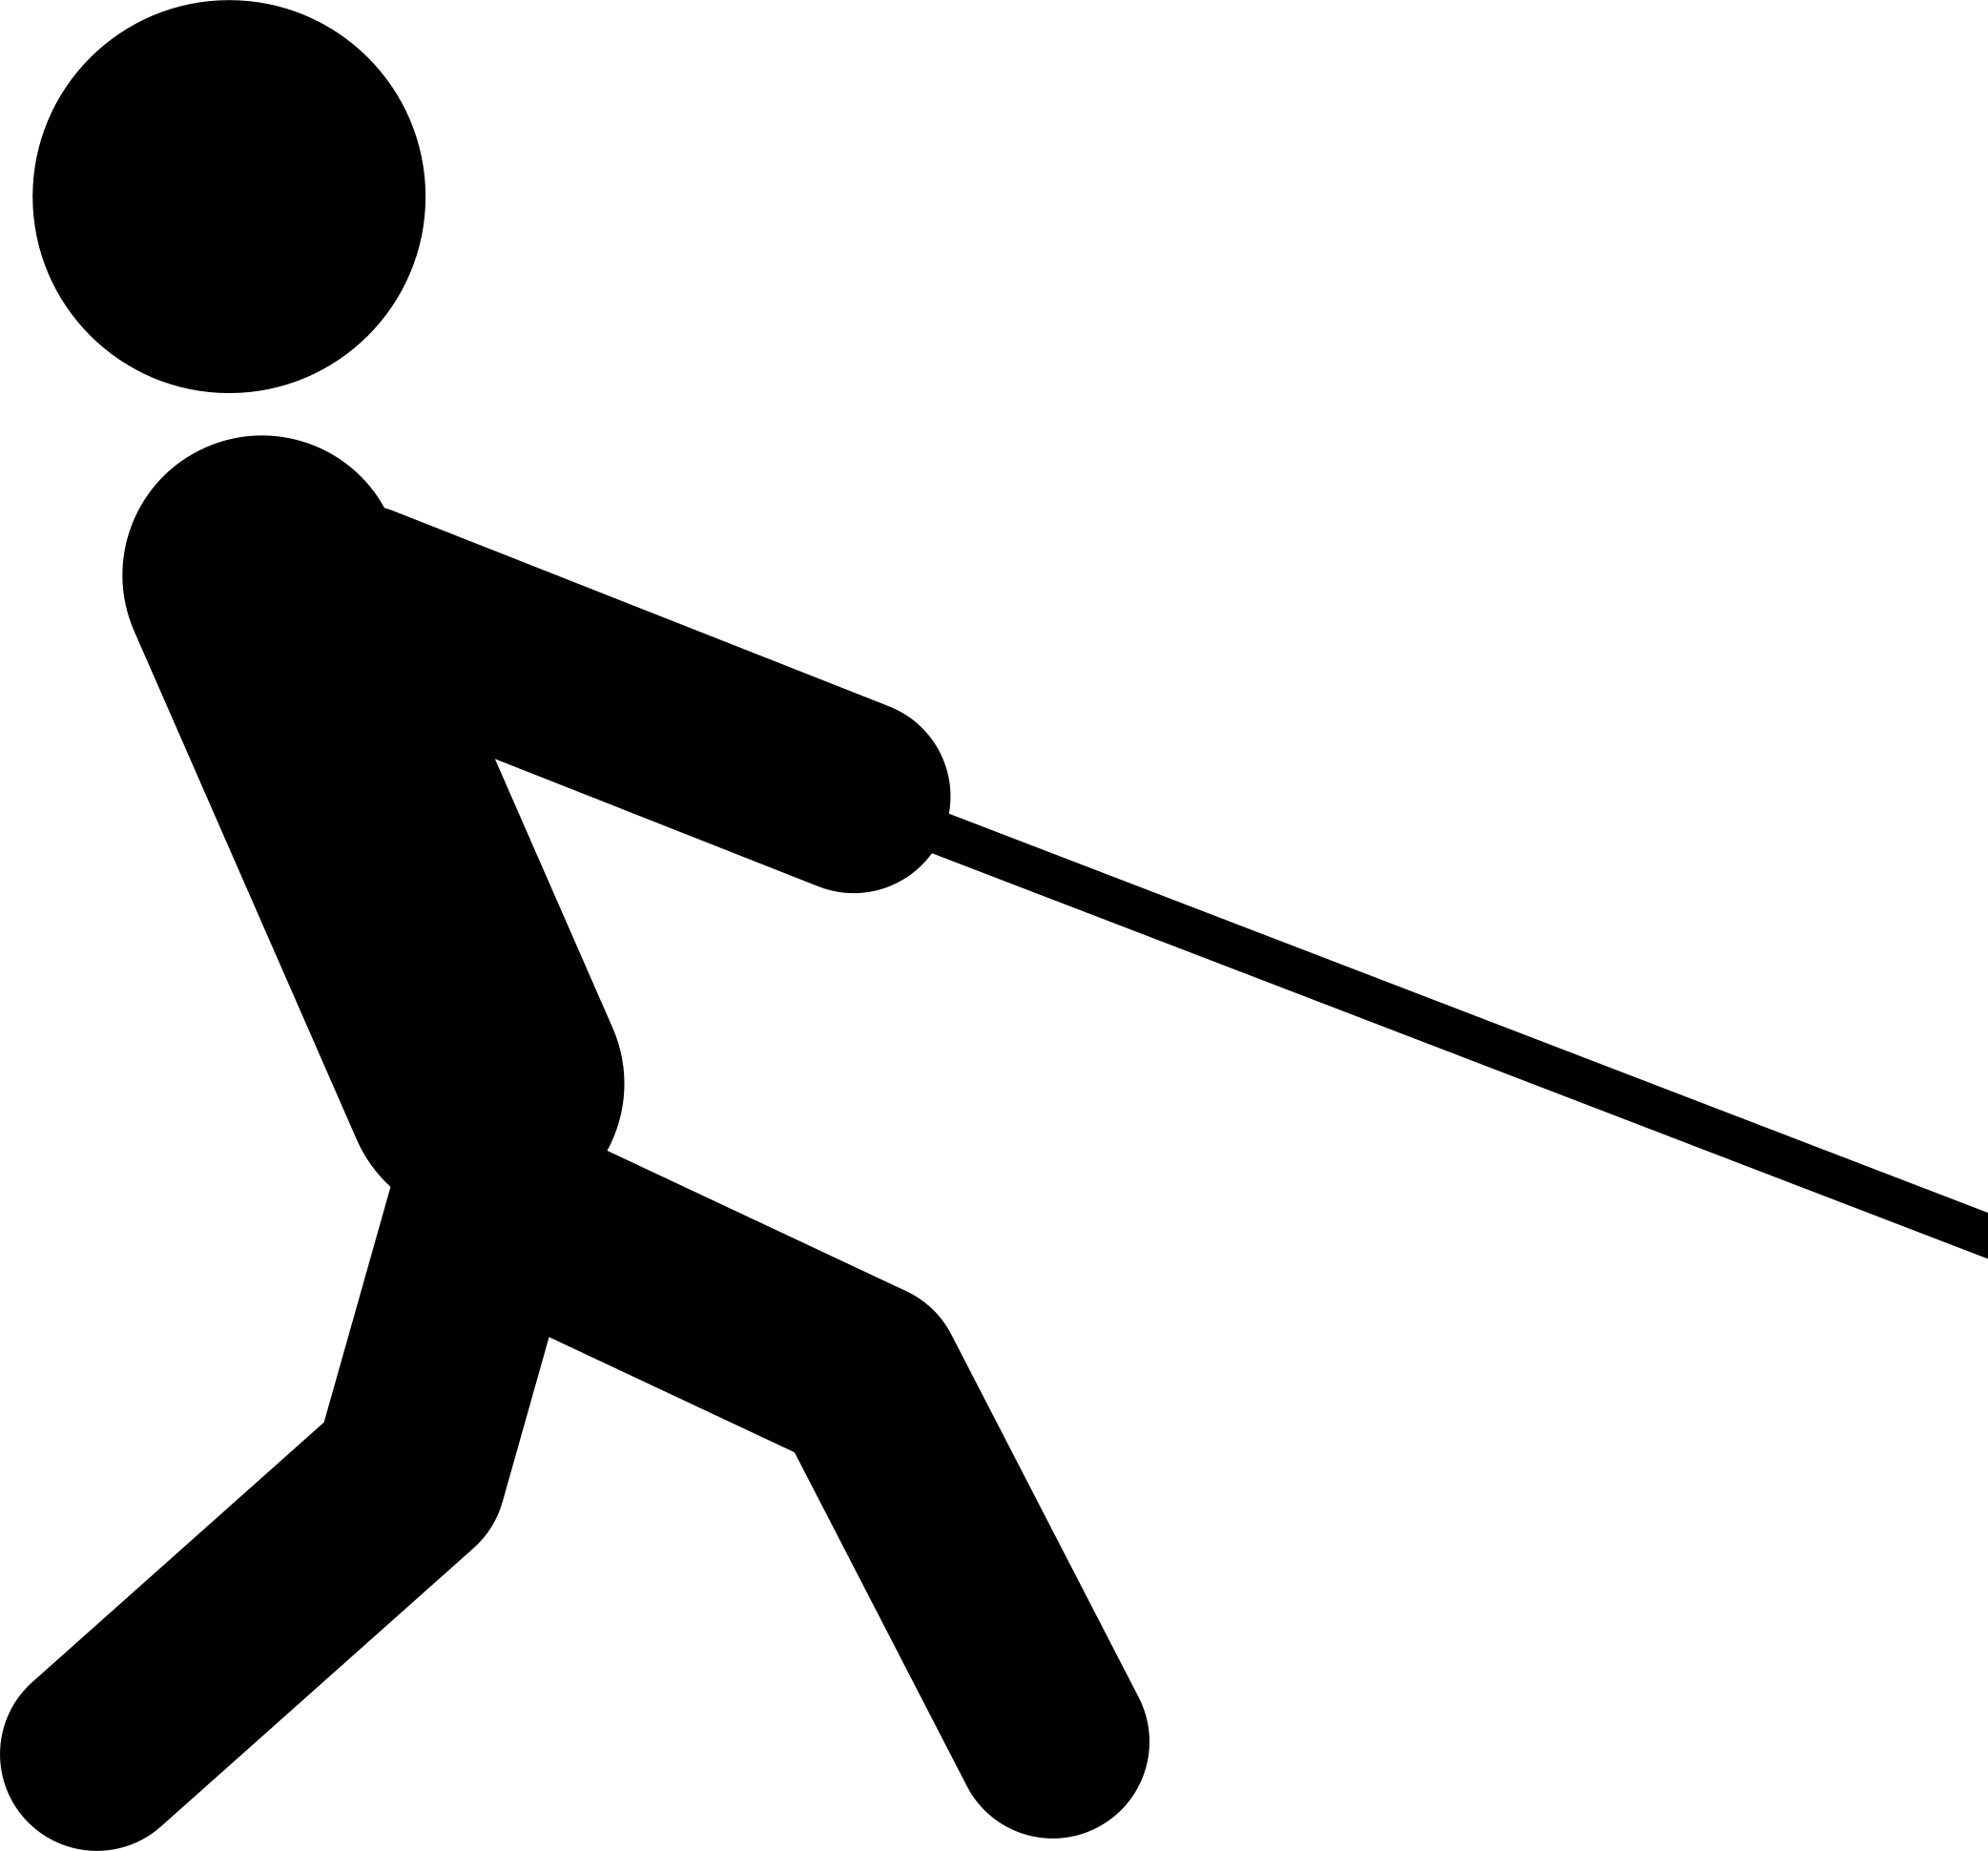
\includegraphics[width=1cm]{clipart/pull}};
\draw[line width=0.6pt] (-0.15,-.15)--(0.75,-.5)--+(0,-3);
\shadedraw[top color=white, bottom color=gray] (-2,-.5)--(.5,-.5)--(.5,-3.5) arc(180:360:2.5mm and 1mm)--(1,-.5)-|(1.5,-4)-|cycle;
\end{tikzpicture}}

\columnbreak
A cable dangles in a hole. The cable is 10 metres long, and has a mass of 5 kg. Its density is constant. We found that the work required to pull the cable out of the hole was
\[25g~J\]
where $g$ is the acceleration due to gravity.
\end{multicols}
\sonslide<3->{
Since the cable has constant density, it should ``balance" at its centre (if it were rigid), so its centre of mass starts 5 metres below the ground. It ends up on the ground. If we treat the cable as a point particle of mass 5 kg, moving against gravity for a distance of 5 metres, we find the work done to be
\[\text{Work}=\text{Force}\cdot\text{distance}=\left(5\, \text{kg}\cdot g\,\frac{\text{m}}{\text{s}^2}\right) \cdot 5\, \text{m}=25g\ J\]
This is much easier than our original calculation.}
\end{frame}
%----------------------------------------------------------------------------------------
\begin{frame}[t]
\AnswerYes<1>\NoSpace<1>
Consider a metre-long rod that is denser on one end than the other, with density
\[\rho(x)=(2x+1)\ \frac{\text{kg}}{\text{m}}\]
at a position $x$ metres from its left end.

\begin{center}\begin{tikzpicture}
\shadedraw[left color=W1!10,right color=W1](0,0)arc(270:90:1mm and 2mm)--(4,.4) arc(90:-90:1mm and 2 mm)--cycle;
\draw (0,0)arc(-90:90:1mm and 2mm);
\xcoord{0}{0} \xcoord{4}{1}
\sonslide<2->{
	\shadedraw[top color=W2, bottom color=W2,middle color=white, ] (.25,0) arc (-90:90:1mm and 2mm)--+(0.2,0) arc (90:-90:1mm and 2mm)--cycle;
	\draw[|-|](.25,-.25)--(.45,-.25)node[midway,below]{$\dee x$};
	 \fill[C3] (2.1,-.5)--(2.3,0)--(2.5,-.5)--cycle;
	}

\end{tikzpicture}\end{center}
What is its centre of mass?\vfill

\sonslide<2->{ We can use our usual slicing-up procedure. Consider slicing the rod into tiny cross-sections, each with width $\dee x$. Then a cross-section at position $x$ is approximately a point mass with position $x$ and mass $\rho(x)\,\dee x = (2x+1)\,\dee x$. So, using integrals to add up the contributions from the different slices, the centre of mass is:
\[\bar x =\frac{\int_0^1 x(2x+1)\ \dee x}{\int_0^1 (2x+1)\ \dee x}=\frac{\left[\frac23x^3+\frac12x^2\right]_0^1}{\left[x^2+x\right]_0^1}=\frac{7/6}{2}=\frac{7}{12}\]
}
\end{frame}
%----------------------------------------------------------------------------------------
\begin{frame}[t]
If a body consists of mass distributed continuously along a straight
line, say with mass density $\rho(x)$kg/m and with $x$ running from $a$ to
$b$, rather than consisting of a finite number of point masses,
the formula for the center of mass becomes
\[
\bar x = \frac{\int_a^b x\ \rho(x)\,\dee{x}}{\int_a^b \rho(x)\,\dee{x}}
\]


\begin{center}\begin{tikzpicture}
\xcoord[below left]{.25}{x}
\xcoord[below right,yshift=1mm]{.45}{x+\dee x}

\shadedraw[left color=W1!10,right color=W1](-1,0)arc(270:90:1mm and 2mm)--(6,.4) arc(90:-90:1mm and 2 mm)--cycle;
\draw (-1,0)arc(-90:90:1mm and 2mm);
\xcoord{-1}{a} \xcoord{6}{b}

\shadedraw[top color=W2, bottom color=W2,middle color=white, ] (.25,0) arc (-90:90:1mm and 2mm)--+(0.2,0) arc (90:-90:1mm and 2mm)--cycle;

\end{tikzpicture}\end{center}

Think of $\rho(x)\,\dee{x}$ as the mass of the ``almost point particle''
between $x$ and $x+\dee{x}$.
\unote{Equation~\eref{text}{eq:TRQvariabledensityrod}}
\end{frame}
%----------------------------------------------------------------------------------------

\begin{frame}[t]
\begin{block}{Centre of Mass}If you support a body at its centre of mass (in a uniform gravitational
field) it balances perfectly. That's the definition of the center of mass
of the body.\end{block}
Centre of mass isn't just for linear solids: it applies to 2- and 3-dimensional objects as well. 

\begin{center}
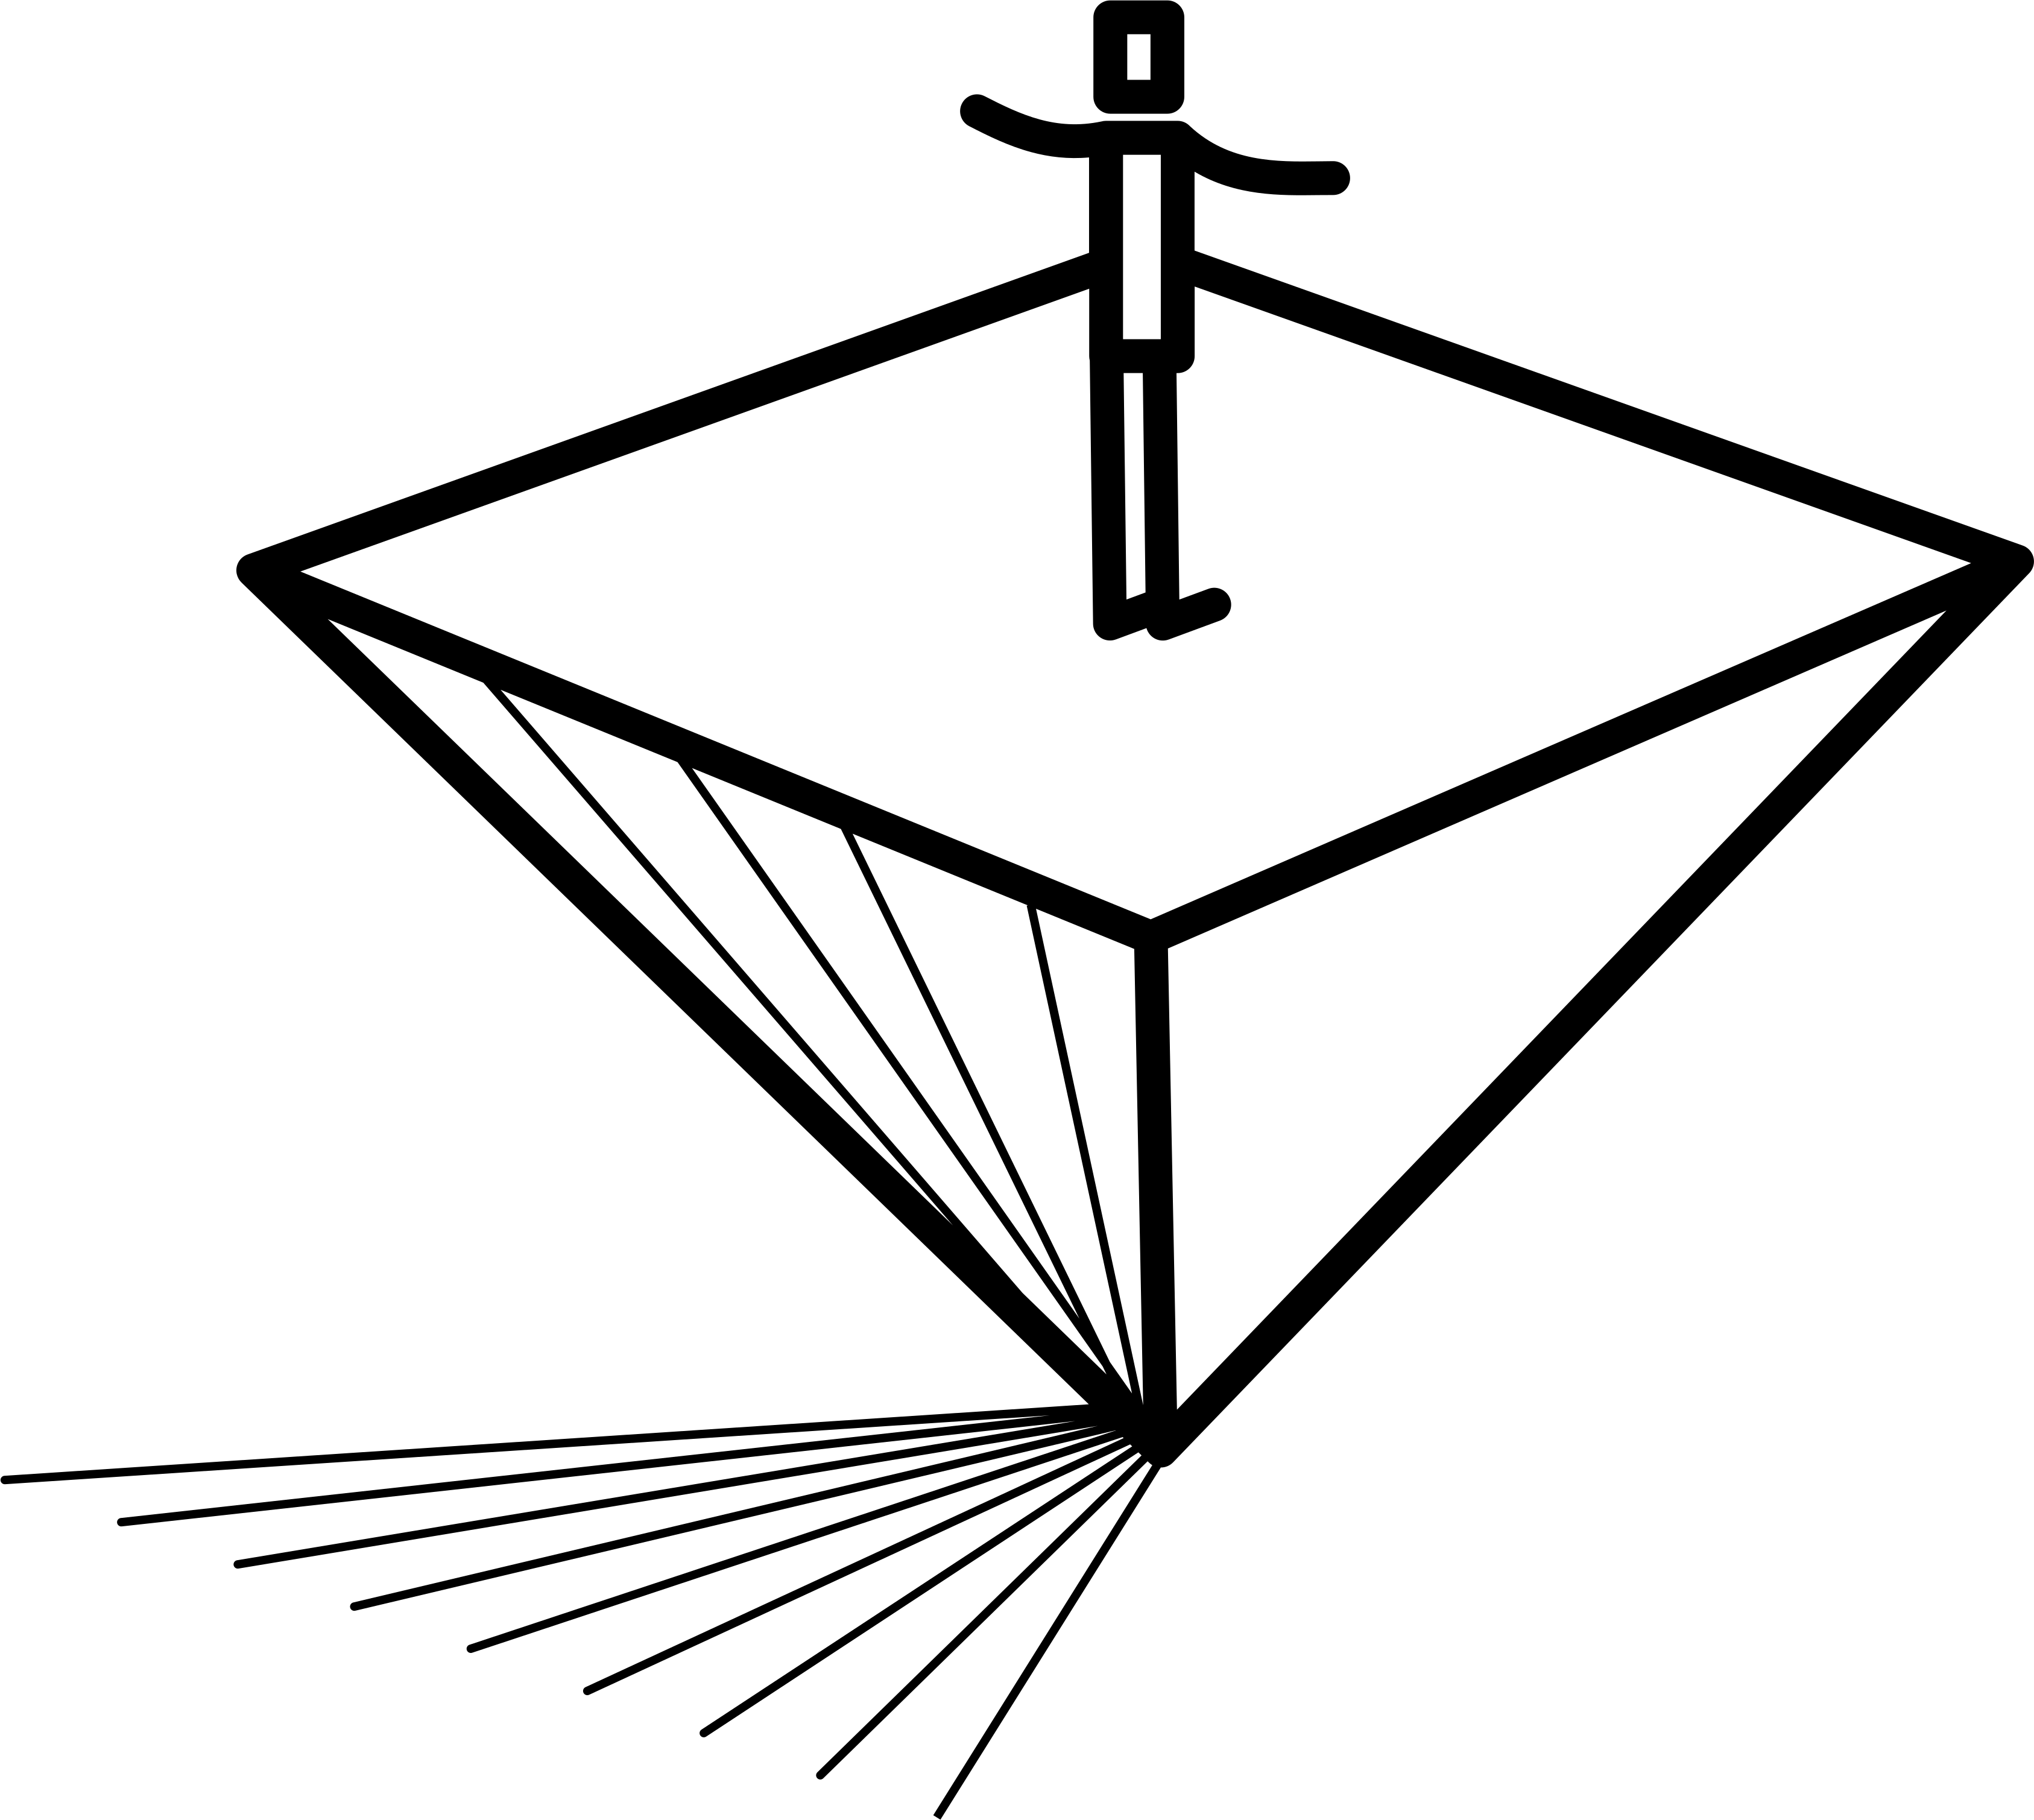
\includegraphics[width=.5\textwidth]{clipart/balancing}
\index{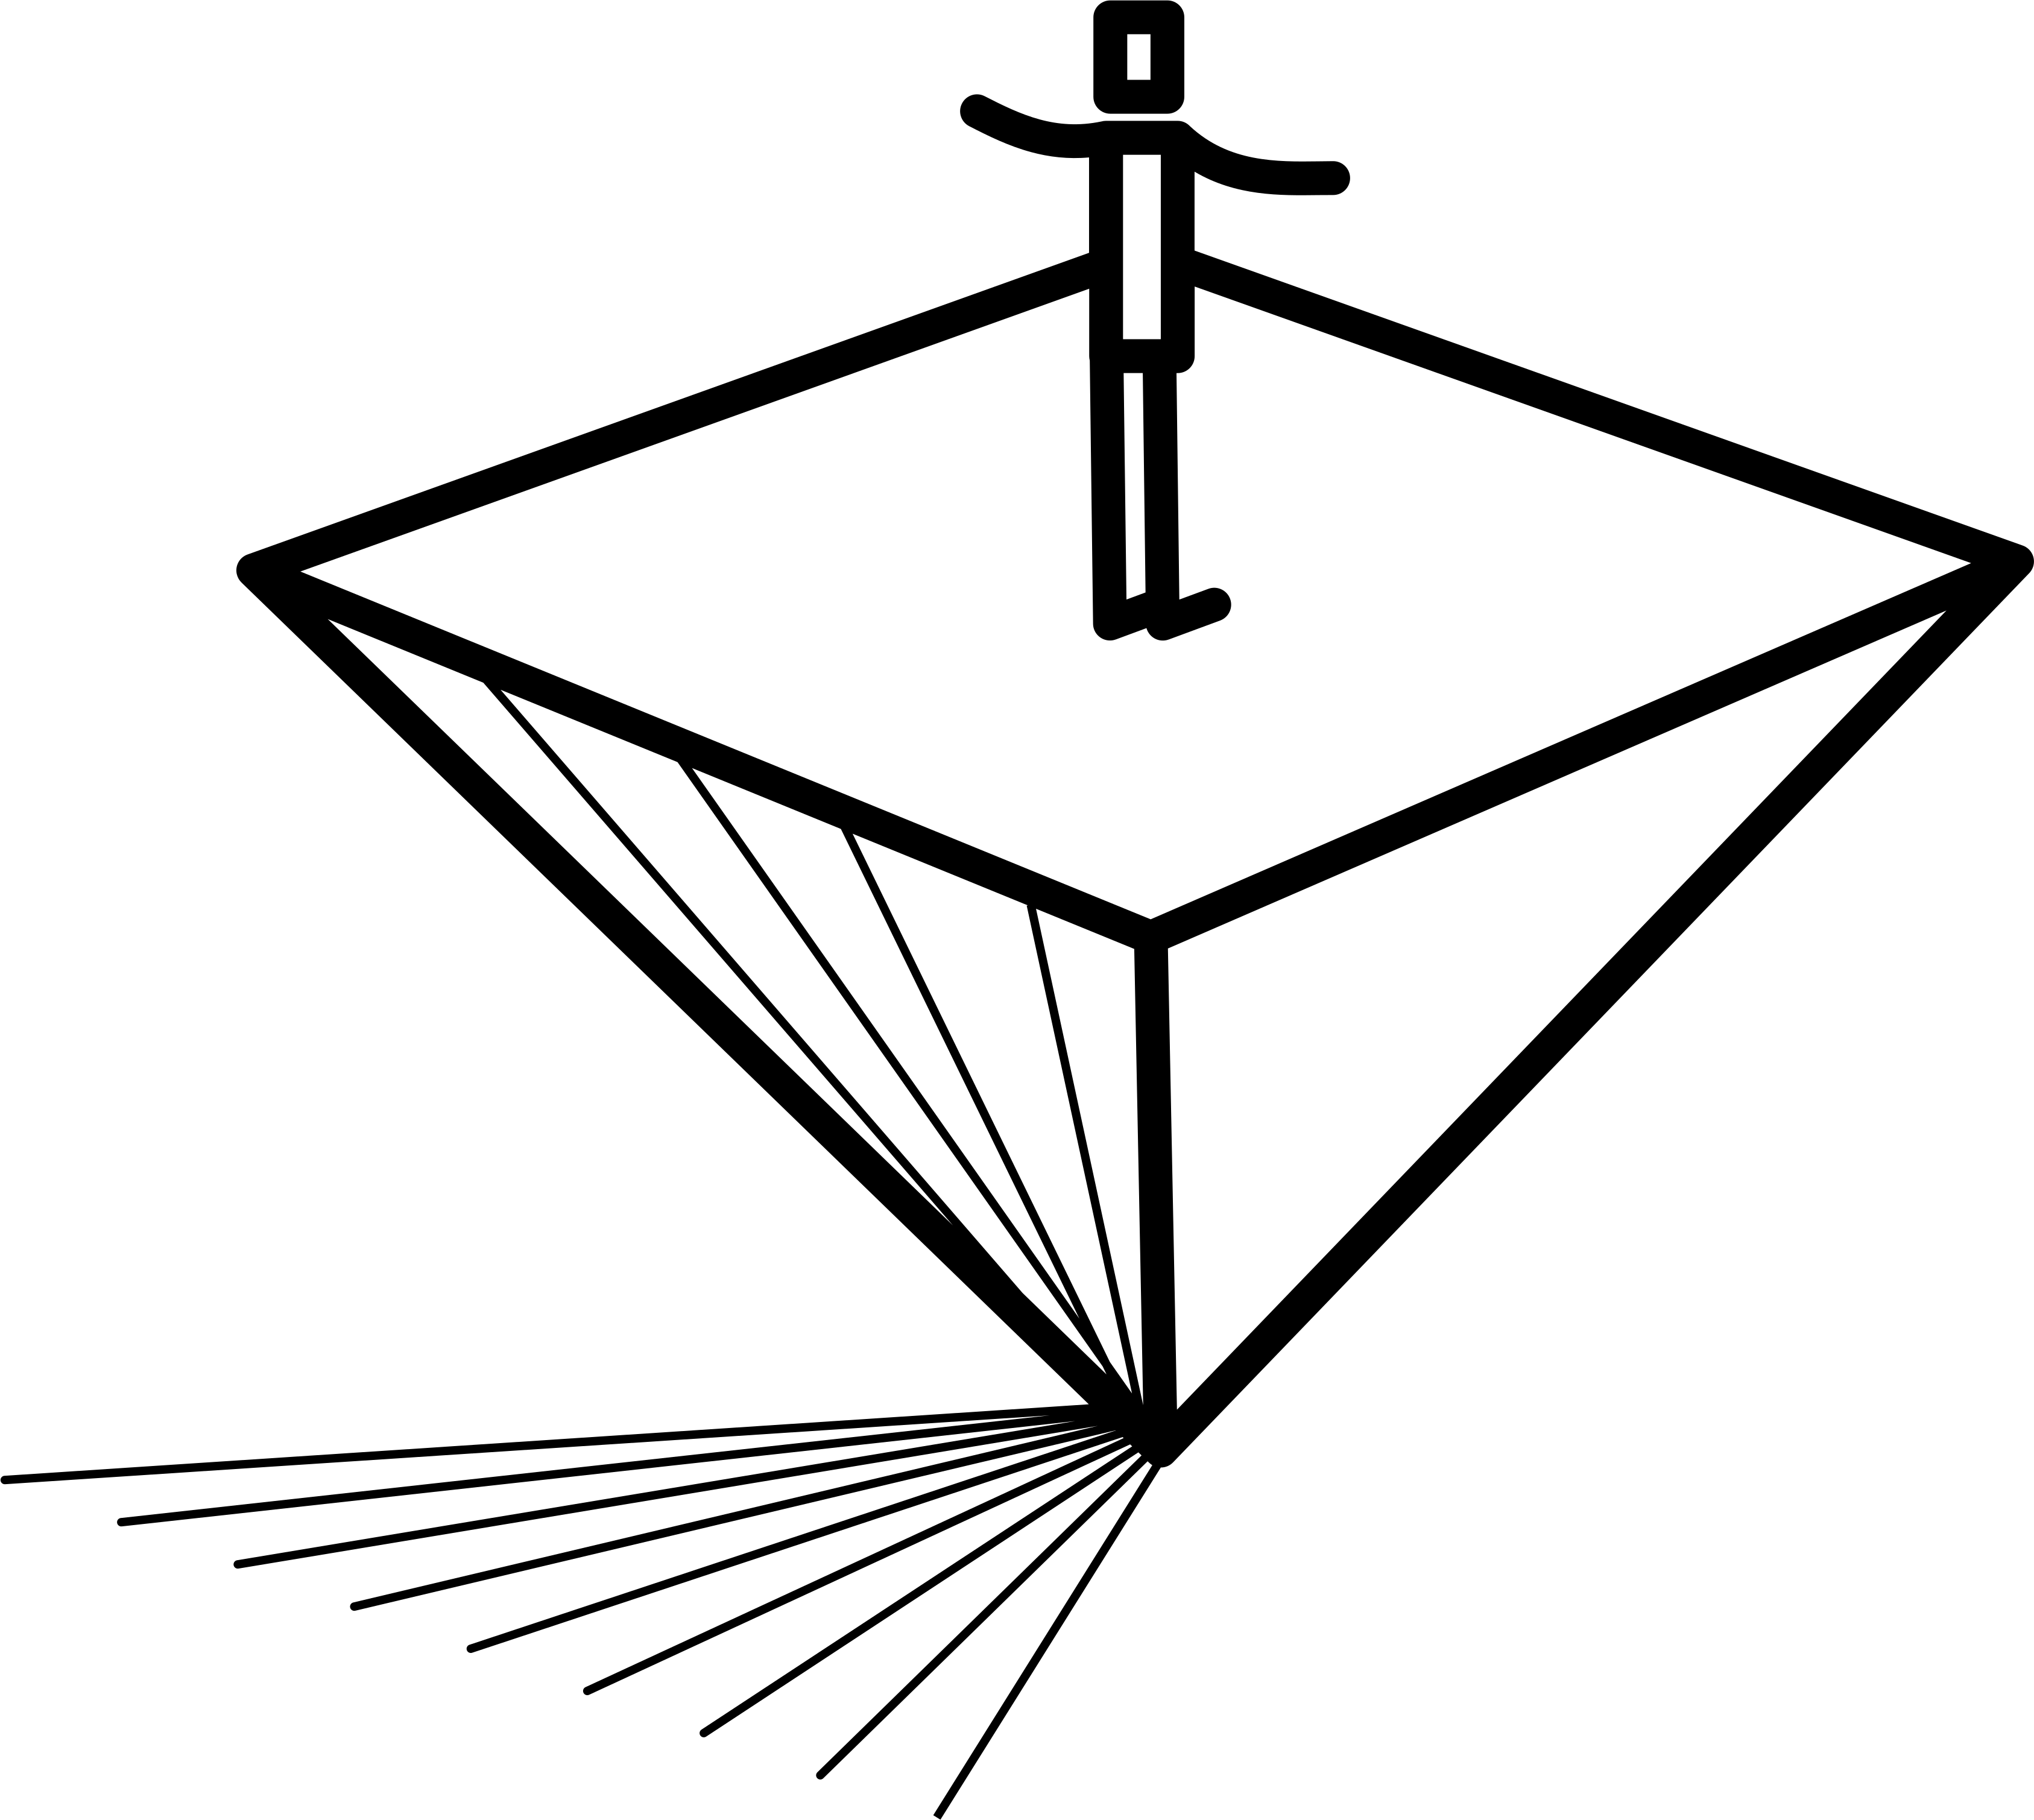
\includegraphics[height=3mm]{clipart/balancing} \href{https://thenounproject.com/icon/balancing-1825102/}{balancing} by \href{https://thenounproject.com/zzyzz/}{Olena Panasovska} is licensed under \CCBYthree~(accessed 10 January 2023)}
\end{center}
\end{frame}
%----------------------------------------------------------------------------------------
\begin{frame}[t]
Consider a flat metal plate of uniform density, whose shape is the area below curve $y=\textcolor{W1}{T(x)}$ and above curve $y=\textcolor{C3}{B(x)}$, from $x=a$ to $x=b$.
\begin{multicols}{2}
\begin{tikzpicture}
\myaxis{x}{0}{4}{y}{0}{3}
\draw[C3, thick] plot[domain=0:4](\x,{\x*\x/5})node[right]{$B(x)$};
\draw[W1, thick] plot[domain=0:4]({\x*\x/4},\x)node[right]{$T(x)$};
\xcoord{1}{a} \xcoord{3}{b}
\fill[C2,opacity=0.5] plot[domain=1:3](\x,{\x*\x/5})--plot[domain=3.46:2]({\x*\x/4},\x)--cycle;

\onslide<3-|handout:0>{
	\filldraw[W2,fill opacity=0.5] plot[domain=1.4:1.6](\x,{\x*\x/5})--plot[domain=2.54:2.37]({\x*\x/4},\x)--cycle;
	\draw[|-|] (1.4,-.5)--(1.6,-.5)node[midway,below]{$\dee x$};
	\draw (1.5,1.5)node[vertex]{};
	}
\end{tikzpicture}\columnbreak

\hfill\parbox{.4\textwidth}{\raggedright\onslide<4-|handout:2>{
If $\rho$ is the density of the plate, so that a slice of width $\dee x$ and height $h=T(x)-B(x)$ has mass $\rho\, h\, \dee x=\rho\big(T(x)-B(x)\big)\,\dee x$, then: \begin{align*}
\bar x &= \frac{\int_a^b \rho(T(x)-B(x))\cdot x\  \dee x}{\int_a^b \rho (T(x)-B(x)) \ \dee x}\\
&=\frac{\int_a^b (T(x)-B(x))\cdot x \ \dee x}{\int_a^b (T(x)-B(x))\ \dee x}
\end{align*}}}
\end{multicols}
The centre of mass will be a point in the $xy$-plane, $(\bar x , \bar y)$.\\ 
\onslide<2->{To find \alert{$\bar x$} and \alert{$\bar y$}, we will treat vertical slices as point particles.}
\end{frame}
%----------------------------------------------------------------------------------------
%----------------------------------------------------------------------------------------
\begin{frame}[t]
\AnswerYes<1>\NoSpace<1>
To find $\bar y$, note that the $y$-coordinate of the centre of mass of a slice that is almost a rectangle, and has uniform density, will be halfway up the slice, at $\frac{T(x)+B(x)}{2}$.
\begin{multicols}{2}
\begin{tikzpicture}
\myaxis{x}{0}{4}{y}{0}{3}
\draw[C3, thick] plot[domain=0:4](\x,{\x*\x/5})node[right]{$B(x)$};
\draw[W1, thick] plot[domain=0:4]({\x*\x/4},\x)node[right]{$T(x)$};
\xcoord{1}{a} \xcoord{3}{b}
\fill[C2,opacity=0.5] plot[domain=1:3](\x,{\x*\x/5})--plot[domain=3.46:2]({\x*\x/4},\x)--cycle;
	\filldraw[W2,fill opacity=0.5] plot[domain=1.4:1.6](\x,{\x*\x/5})--plot[domain=2.54:2.37]({\x*\x/4},\x)--cycle;
	\draw[|-|] (1.4,-.5)--(1.6,-.5)node[midway,below]{$\dee x$};
	\draw (1.5,1.5)node[vertex]{};
\ycoord{1.5}{\frac{T(x)+B(x)}{2}}
\end{tikzpicture}\columnbreak

$ $
\vspace{7mm}\onslide<2-|handout:2>{
 \begin{align*}
\bar y &= \frac{\int_a^b  \left(\frac{T(x)+B(x)}{2}\right) \cdot \rho(T(x)-B(x))\  \dee x}{\int_a^b \rho (T(x)-B(x)) \ \dee x}\\
&=\frac{\frac12\int_a^b (T^2(x)-B^2(x)) \ \dee x}{\int_a^b (T(x)-B(x))\ \dee x}
\end{align*}}
\end{multicols}
\end{frame}
%----------------------------------------------------------------------------------------
\begin{frame}[t]
\AnswerYes<1>\NoSpace<1>

  Find the centre of mass (centroid) of the quarter circular unit disk $x\ge 0$,
$y\ge 0$, $x^2+y^2\le 1$.

\begin{multicols}{2}


\begin{tikzpicture}
\myaxis{x}{0}{2.2}{y}{0}{2.2}
\filldraw[C1,fill=C2,fill opacity=0.5] (2,0) arc (0:90:2cm)|-cycle;
\sonslide<2->{\draw (.85,.85)node[vertex]{};\xcoord{.85}{\frac{4}{3\pi}} \ycoord{.85}{\frac{4}{3\pi}}}
\end{tikzpicture}

\sonslide<2->{
 By symmetry, $\bar x=\bar y$. Using the equations we developed above with top $y=T(x)=\sqrt{1-x^2}$ and bottom $y=B(x)=0$:
 
\begin{align*}
\bar x & = \frac{\int_0^1 (\sqrt{1-x^2}-0)\cdot x\, \dee x}{\int_0^1 (\sqrt{1-x^2}-0)\, \dee x}
\intertext{For the integral in the numerator, let $u=1-x^2$, $\dee u = -2x \ \dee x$. The denominator is the area of the quarter unit circle.}
&=\frac{\int_1^0 -\frac12 u^{1/2}\ \dee u}{\frac{\pi}{4}}\\
&=\frac{2}{\pi}\int_0^1u^{1/2}\ \dee u\\
&=\frac{2}{\pi}\left[\frac{2}{3}u^{3/2}\right]_0^1
=\frac{4}{3\pi}\\
(\bar x , \bar y )&=\left(\frac{4}{3\pi},\frac{4}{3\pi}\right)
\end{align*} }

\end{multicols}
\unote{Example~\eref{text}{eg:TRQcentroidBa}}
\end{frame}
%----------------------------------------------------------------------------------------
\begin{frame}[t]
\AnswerYes<1>\NoSpace<1>
\sStatusBar{1}{5}
 Find the centre of mass (centroid) of a plate of uniform density in the shape of the finite area enclosed by the functions $y=T(x)=2-x$ and $y=B(x)=x^2$.
\begin{multicols}{2}
\begin{tikzpicture}
\myaxis{x}{2.2}{2.2}{y}{0}{4.2}
\draw[W1,thick] plot[domain=-2.1:2](\x,{2-\x});
\draw[C1,thick] plot[domain=-2.1:2.1,smooth](\x,{\x*\x});
\fill[C2,opacity=0.5] plot[domain=--2:1](\x,{2-\x})-- plot[domain=1:-2](\x,{\x*\x})--cycle;

\sonslide<2->{	\xcoord{-2}{-2}	\xcoord{1}{1}}
\sonslide<4->{\xcoord{-.5}{-\frac12}}
\sonslide<5->{\nycoord[fill=white,fill opacity=0.75]{1.6}{\frac{8}{5}}
	\draw(-.5,1.6)node[vertex]{};}
\end{tikzpicture}\columnbreak

\sonly<2>{
First, we find where the curves intersect.
\begin{align*}
x^2&=2-x\\
x^2+x-2&=0\\
(x-1)(x+2)&=0\\
x&=-2,\ x=1
\end{align*}
}
\sonly<3>{
The denominator is the same in our $\bar x$ and $\bar y$ calculations, so let's find that next.
\begin{align*}
&\int_{-2}^1\!\!\! \left(T(x)-B(x)\right)\dee x =\!\!\! \int_{-2}^1\!\!\! \left(2-x-x^2\right)\dee x \\
& =\left[2x-\frac{1}{2}x^2-\frac13x^3\right]_{-2}^1\\
&=\left(2-\frac12-\frac13\right)-\left(-4-2+\frac{8}{3}\right)\\
&=\frac{9}{2}
\end{align*}
}
\sonly<4>{
\begin{align*}
\bar x&=\frac{\int_{-2}^1 \left(2-x-x^2\right)x \ \dee x}{\int_{-2}^1 \left(2-x-x^2\right)\ \dee x }\\
&=\frac{\int_{-2}^1 \left(2x-x^2-x^3\right) \ \dee x}{\frac92}\\
&=\frac29\left[x^2-\frac13x^3-\frac14x^4\right]_{-2}^1\\
&=\frac29\left[\left(1-\frac13-\frac14\right)-\left(4+\frac83-4\right)\right]\\
&=-\frac12
\end{align*}
}
\sonly<5>{
\begin{align*}
\bar y&=\frac{\frac12\int_{-2}^1 \left((2-x)^2-(x^2)^2\right)x \ \dee x}{\int_{-2}^1 \left(2-x-x^2\right)\ \dee x }\\
&=\frac{\frac12\int_{-2}^1\left( 4-4x+x^2-x^4\right)\dee x}{\frac{9}{2}}\\
&=\frac19\left[4x-2x^2+\frac13x^3-\frac15x^5 \right]_{-2}^1\\
&=\frac19\Big[\left(4-2+\frac13-\frac15\right)\\&\qquad-\left(-8-8-\frac83+\frac{32}{5}\right)\Big]=\frac{8}{5}
\end{align*}
}
\end{multicols}
\end{frame}
%----------------------------------------------------------------------------------------
%----------------------------------------------------------------------------------------

